\date{}
\title{}
\date{}
\begin{document}
\begin{frame}
    \titlepage
\end{frame}


\makeatletter
\newenvironment<>{btHighlight}[1][]
{\begin{onlyenv}#2\begingroup\tikzset{bt@Highlight@par/.style={#1}}\begin{lrbox}{\@tempboxa}}
{\end{lrbox}\bt@HL@box[bt@Highlight@par]{\@tempboxa}\endgroup\end{onlyenv}}

\newcommand<>\btHL[1][]{%
  \only#2{\begin{btHighlight}[#1]\bgroup\aftergroup\bt@HL@endenv}%
}
\def\bt@HL@endenv{%
  \end{btHighlight}%   
  \egroup %
}
\tikzset{
    btHLbox/.style={
        fill=red!30,outer sep=0pt,inner xsep=1pt, inner ysep=0pt, rounded corners=3pt
    },
}
\newcommand{\bt@HL@box}[2][]{%
  \tikz[#1]{%
    \pgfpathrectangle{\pgfpoint{1pt}{0pt}}{\pgfpoint{\wd #2}{\ht #2}}%
    \pgfusepath{use as bounding box}%
    \node[text width={},draw=none,anchor=base west, btHLbox, minimum height=\ht\strutbox+1pt,#1]{\raisebox{1pt}{\strut}\strut\usebox{#2}};
  }%
}

\lst@CCPutMacro
    \lst@ProcessOther {"2A}{%
      \lst@ttfamily 
         {\raisebox{2pt}{*}}% used with ttfamily
         {\raisebox{2pt}{*}}}% used with other fonts
    \@empty\z@\@empty

\lstdefinelanguage
   [x8664gas]{Assembler}     % add a "x64" dialect of Assembler
   [x86masm]{Assembler} % based on the "x86masm" dialect
   % with these extra keywords:
   {morekeywords={CDQE,CQO,CMPSQ,CMPXCHG16B,JRCXZ,LODSQ,MOVSXD,%
                  POPFQ,PUSHFQ,SCASQ,STOSQ,IRETQ,RDTSCP,SWAPGS,.TEXT,.STRING,.ASCIZ,%
                  BEQ,LW,SW,LB,SB,ADDIU,J,BEQZ,BNEZ,BNE,%
                  MOVUPD,MULPD,MOVSD,MULSD,%
                  SHLADD,MOV,CMP.LT,TBIT.NZ,BR.RET.SPTK.MANY,%
                  ADDQ,POPQ,PUSHQ,RRMOVQ,MRMOVQ,RMMOVQ,IRMOVQ,%
                  <-,LL,SC,ADDI,ADDL,VMOVDQA,ADDQ,CMPL,JB,JBE,MOVL,CLTQ,
                  MOVW,PUSHW,MOV,ADD,SUB,INT,PUSH,MOV,ADD,REP,MOVSB,%
                  TESTQ,CMPQ,MOVL,MOVQ,ADDQ,JMPQ,XORQ,%
                  LEAQ,LEAL,LEA,RETQ,RET,POPL,POPW,PUSHL,PUSHW,%
                  LEAW,%
                  SUBQ,SYSCALL,.ASCII,CALLQ,MOVSLQ,JMP,ANDQ,SHRQ,MOVB,INCQ,TESTL,XORL,%
                  SHRL,LEAL,SARL,SUBL,IMULL,IMULQ,MOVDQU,PADDD,XORL,%
                  MOVZBL,MOVZB,SHRB,SRAL,SHRL,ANDL,%
                  CMOVNS,SRAL,SRAQ,MOVZBW,MOVZBQ,%
                  PADDW,PADDQ,MODUPS,MOVAPD,%
                  MOVL,RET,.GLOBL,%
                  },
    deletekeywords={eax,ebx,sp,si,cx,di,ds,cs,es,fs,dx,ax,bx,al,esi,ebp,ecx,rip,eip,edx,edi,rdi,esp},
    morecomment=[l]{\#},
    morecomment=[l]{\/\/},
    morecomment=[s]{/*}{*/},
    sensitive=false,
    keepspaces=true} % et

\lstalias[]{myasm}[x8664gas]{Assembler}

\lstdefinelanguage{JavaScript}{
  keywords={typeof, new, true, false, catch, function, return, null, catch, switch, var, if, in, while, do, else, case, break},
  ndkeywords={class, export, boolean, throw, implements, import, this},
  sensitive=false,
  comment=[l]{//},
  morecomment=[s]{/*}{*/},
  morestring=[b]',
  morestring=[b]"
}

\newcommand{\keywordstyle}{\sourcecodeprolight\bfseries\color{blue!30!black}}
\newcommand{\stringstyle}{\color{blue!20!black}\ttfamily}

\lstset{
    language=C,
    basicstyle=\sourcecodepro\EmptyMapping,
    escapechar=`,
    keywordstyle=\keywordstyle\EmptyMapping,
    identifierstyle=\sourcecodepro\EmptyMapping,
    numberstyle=\small\color{black!70},
    commentstyle=\color{red!60!black}\ttfamily\itshape,
    stringstyle=\color{blue!20!black}\ttfamily,
    ndkeywordstyle=\bfseries\color{blue!30!black},
    upquote=true,
}



\lstdefinestyle{medium}{
    basicstyle=\sourcecodepro\EmptyMapping\fontsize{12}{13}\selectfont,
    keywordstyle=\sourcecodepro\EmptyMapping\fontsize{12}{13}\selectfont\keywordstyle,
}

\lstdefinestyle{small}{
    basicstyle=\sourcecodepro\EmptyMapping\small,
    keywordstyle=\sourcecodepro\EmptyMapping\small\keywordstyle,
}

\lstdefinestyle{smaller}{
    basicstyle=\sourcecodepro\EmptyMapping\fontsize{11}{12}\selectfont,
    keywordstyle=\sourcecodepro\EmptyMapping\fontsize{11}{12}\selectfont\keywordstyle,
}


\lstdefinestyle{script}{
    basicstyle=\sourcecodepro\EmptyMapping\scriptsize,
    keywordstyle=\sourcecodepro\EmptyMapping\scriptsize\bfseries,
}




\begin{frame}{last time}
    \begin{itemize}
    \item copy-on-write, page table tricks
        \begin{itemize}
        \item react to page/protection fault by filling in table
        \item separate data structure --- Linux: `maps' list
        \end{itemize}
    \item storing page tables in memory
        \begin{itemize}
        \item encoding as array of integers
        \item special register pointing to base of array
        \end{itemize}
    \item multi-step page table access
        \begin{itemize}
        \item two memory accesses / program access
        \end{itemize}
    \end{itemize}
\end{frame}

\begin{frame}{quiz Q4}
    \begin{itemize}
    \item memory access steps:
    \vspace{.5cm}
    \item virtual address $\rightarrow$ virtual page number (VPN) | page offset (PO)
    \item read page table entry at BASE + VPN $\times$ entry size
        \begin{itemize}
        \item<2-> \myemph{\texttt{0x100000} + VPN $\times$ 8 = \texttt{0x100340}}
        \end{itemize}
    \item decode page table entry to get valid  + permission + PPN
        \begin{itemize}
        \item<2-> \myemph{\texttt{0x400000F} $\rightarrow$ valid, all perms, PPN 0x4000}
        \end{itemize}
    \item access memory for program at PPN [concat] PO
    \end{itemize}
\end{frame}

\begin{frame}{quiz Q4 (2)}
    \begin{itemize}
    \item no restrictions on page offset
    \item VPN satisfies {\tt 0x100000} + VPN $\times$ 8 = \texttt{0x100340}
    \item $\rightarrow$ VPN = 0x68
    \item virtual address $\rightarrow$ 0x68 | page offset (12-bit)
    \item \texttt{0x68xxx} [any 12 bits in xxx]
    \end{itemize}
\end{frame}

\section{handling big page tables}
\subsection{general options}
\usetikzlibrary{patterns,positioning,calc,fit}

\begin{frame}{huge page tables}
\begin{itemize}
    \item huge virtual address spaces!
    \item impossible to store PTE for every page
    \vspace{.5cm}
    \item how can we save space?
\end{itemize}
\end{frame}

\begin{frame}{holes}
\begin{tikzpicture}
\tikzset{
    mylabel/.style={font=\ttfamily},
    mybox/.style={draw,rectangle,minimum width=7cm,fill=white,inner sep=1mm},
    myhigh/.style={draw,rectangle,line width=1mm, draw=blue!80!black,opacity=.3},
}
\begin{scope}[name prefix=A-]
\node[mybox,minimum height=1cm,pattern=north west lines,pattern color=black!5!white] (kernel) {Used by OS};
\node[mybox, minimum height=.5cm, below=1cm of kernel] (stack) {Stack};
\node[mybox, minimum height=.5cm, below=1cm of stack] (heap) {Heap / other dynamic};
\node[mybox, minimum height=.5cm, below=0mm of heap] (data) {Writable data};
\node[mybox, minimum height=.5cm, below=0mm of data] (sdata) {Code + Constants};
\coordinate (memBottom) at ($(sdata.south east) + (0mm, -2mm)$);
\begin{pgfonlayer}{bg}
\draw[pattern=north west lines, pattern color=black!40!white] (kernel.north west) rectangle (memBottom);
\end{pgfonlayer}
\node[fill=red,fill opacity=0.05,inner sep=0mm,draw=red,ultra thick,fit=(kernel.south west) (stack.north east)] {};
\node[fill=red,fill opacity=0.05,inner sep=0mm,draw=red,ultra thick,fit=(stack.south west) (heap.north east)] {};
\node[fill=red,fill opacity=0.05,inner sep=0mm,draw=red,ultra thick,fit=(sdata.south west) (memBottom)] {};
\end{scope}
\node[right=1cm of A-stack] {most pages are \myemph{invalid}};
\end{tikzpicture}
\end{frame}

\begin{frame}{saving space}
\begin{itemize}
    \item basic idea: don't store (most) invalid page table entries
    \item use a data structure other than a flat array
        \begin{itemize}
        \item want a map --- lookup key (virtual page number), get value (PTE)
        \end{itemize}
    \item options?
    \vspace{.5cm}
    \item<2-> \myemph<2>{hashtable}
        \begin{itemize}
        \item<2-> actually used by some historical processors
        \item<2-> but never common
        \end{itemize}
    \item<3-> \myemph<3>{tree data structure}
        \begin{itemize}
        \item<3-> but not quite a search tree
        \end{itemize}
\end{itemize}
\end{frame}

\begin{frame}{search tree tradeoffs}
    \begin{itemize}
    \item lookup usually implemented \myemph{in hardware}
        \begin{itemize}
        \item lookup should be simple
        \item solution: lookup splits up address bits (no complex calculations)
        \end{itemize}
    \item lookup should not involve many memory accesses
        \begin{itemize}
        \item doing two memory accesses is already very slow
        \item solution: tree with many children from each node
            \begin{itemize}
            \item (far from binary tree's left/right child)
            \end{itemize}
        \end{itemize}
    \end{itemize}
\end{frame}



\subsection{two-level page tables}
\usetikzlibrary{arrows.meta, fit}
\begin{frame}<0>[label=twoLevelPtLookup]{two-level page table lookup}
\begin{tikzpicture}
\tikzset{
    >=Latex,
    pageNumber/.style={fill=blue!10,font=\fontsize{11}{12}\selectfont,inner sep=.5mm},
    pageNumberA/.style={fill=violet!30,font=\fontsize{11}{12}\selectfont,inner sep=.5mm,draw,thick,dotted},
    pageNumberB/.style={fill=brown!20,font=\fontsize{11}{12}\selectfont,inner sep=.5mm,draw,thick,dotted},
    pageOffset/.style={fill=green!20,font=\fontsize{11}{12}\selectfont,inner sep=.5mm},
    comp/.style={fill=yellow!10,font=\fontsize{11}{12}\selectfont,draw},
    memAccess/.style={alt=<all:7>{red, very thick}},
    pageNumberExpand/.style={alt=<all:11>{draw=red,very thick}},
    smallLabel/.style={fill=white,draw,thick,font=\fontsize{10}{11}\selectfont,inner sep=.5mm,align=center},
}
\node[pageNumberA] (addrLeftA) {11 0101 01};
\node[pageNumberB,anchor=west] (addrLeftB) at (addrLeftA.east) {00 1011 00};
\node[anchor=west,pageOffset] (addrRight) at (addrLeftB.east) {00 1101 1111};
\node[inner sep=0mm,draw=none,fit=(addrLeftA) (addrLeftB),alt=<1>{draw=red,very thick}] (addrLeft) {};
\begin{visibleenv}<all:1>
\node[below=1cm of addrLeft,xshift=2cm] (vpn split explain) {VPN --- split into two parts (one per level)};
\node[below=1cm of vpn split explain,font=\small] {
    this example: parts equal sized --- common, but not required
};
\end{visibleenv}
\begin{visibleenv}<all:2->
\node[draw,comp,below=1cm of addrLeftA,align=center,xshift=-1cm] (timesPte) {$\times$ \\ PTE \\ size};
\draw[->,thick] (addrLeftA) -- ++(0cm,-.5cm) -| (timesPte);
\node[font=\tt\fontsize{10}{11}\selectfont,draw,very thick,left=0.25cm of addrLeft,label={[align=center,font=\small]north:page table\\base register},yshift=-.5cm] (ptbr) {0x10000};
\node[draw,comp] (plus) at ([yshift=-1cm]timesPte.south) {+};
\draw[->,thick] (timesPte) -- (plus);
\draw[->,thick] (ptbr) |- (plus);
\end{visibleenv}

\begin{visibleenv}<all:3->
\node[below=1.5cm of plus,fill=violet!10,draw,very thick,minimum height=1cm,minimum width=15cm,xshift=5.5cm] (cache) {memory {\small (really cache)}};
\end{visibleenv}
\begin{visibleenv}<all:5->
\node[pageNumber] (addrLeftFinal) at ([xshift=9.6cm,yshift=-1cm]plus) {1101 0011 11};
\end{visibleenv}
\begin{visibleenv}<all:3->
\draw[->,thick,memAccess] (plus) -- (cache.north -| plus.south) node[midway,smallLabel] {1st PTE \\ addr.};
\node[above right=1cm and .5cm of plus,align=center,draw,comp,font=\small] (check) {valid, etc?};
\node[below=.75cm of check,draw,comp,align=center] (splitA) {split  \\ PTE parts};
\draw[->,thick] (cache.north -| splitA.south) -- (splitA.south);
\draw[->,thick] (splitA) -- (check);
\draw[->,thick] (check.north) -- ++(0,.75cm) node[above,font=\small,inner sep=.5mm] {cause fault?};
\end{visibleenv}

\begin{visibleenv}<all:4->
    \node[comp,align=center,right=.75cm of splitA,pageNumberExpand] (timesSize){$\times$ \\ page \\ size};
    \node[comp,align=center,right=1.25cm of timesSize] (plusB) {+};
    \draw[brown!60!black,->,thick,pageNumberExpand] (splitA) -- (timesSize);
    \draw[dotted,black,thick] ($(splitA.east)!0.5!(timesSize.west)$) -- ++ (0cm, .5cm) node[above,font=\fontsize{10}{11}\selectfont,align=center] {phys\\page \#};
    \draw[brown!60!black,->,thick,pageNumberExpand] (timesSize) -- (plusB);
    \draw[dotted,black,thick] ($(plusB.east)!0.5!(timesSize.west)$) -- ++ (0cm, .5cm) node[above,font=\fontsize{10}{11}\selectfont,align=center] {phys\\addr};
    \draw[memAccess,->,thick] (plusB) -- (plusB |- cache.north) node[midway,smallLabel]{2nd PTE \\ addr.};
    \node[comp,align=center,above=.5cm of plusB] (timesPteB) {$\times$ \\ PTE \\ size};
    \draw[brown!60!black,->,thick] (addrLeftB) -- ++(0cm,-.5cm) -| (timesPteB.north);
    \draw[brown!60!black,->,thick] (timesPteB) -- (plusB);
\end{visibleenv}

\begin{visibleenv}<all:5->
\node[right=.5cm of plusB,draw,comp,align=center] (splitB) {split  \\ PTE parts};
\draw[->,thick] (cache.north -| splitB.south) -- (splitB.south);
\node[above=.75cm of splitB,align=center,draw,comp,font=\small] (checkB) {valid, etc?};
\draw[->,thick] (splitB) -- (checkB);
\draw[->,thick] (checkB.north) -- ++(0cm, .75cm) node[above,font=\small,inner sep=.5mm] {cause fault?};
\draw[blue!50!black,->,thick] (splitB) -| (addrLeftFinal);
\end{visibleenv}

\begin{visibleenv}<all:6->
\node[anchor=west,pageOffset] (addrRightFinal) at (addrLeftFinal.east) {00 1101 1111};
%\draw[very thick,green!50!black,densely dotted] (addrRight) |- ([xshift=-.5mm,yshift=.5cm]splitA.north);
\draw[very thick,green!50!black,densely dotted,->] (addrRight) -| (addrRightFinal.north);
\end{visibleenv}
\begin{visibleenv}<all:3->
\node[inner sep=0mm,draw,label={[font=\fontsize{12}{13}\selectfont]south:physical address},fit=(addrLeftFinal) (addrRightFinal)] (addrFinal) {};
\end{visibleenv}

\node[inner sep=0mm,draw,label={[font=\fontsize{12}{13}\selectfont]north:virtual address},fit=(addrLeft) (addrRight)] (addr) {};
\begin{visibleenv}<all:5->
    \draw[->,thick,memAccess] (addrFinal) -- (cache.north -| addrFinal.south);
\end{visibleenv}

\begin{pgfonlayer}{bg}
\begin{visibleenv}<all:8,10>
    \node [fill=violet!5,fit=(timesPte) (splitA),draw,line width=0.125mm,dashed] (firstBox) {};
\end{visibleenv}
\begin{visibleenv}<all:9,10>
    \node [fill=brown!5,fit=(timesPteB) (splitB),draw,line width=0.125mm,dashed] (secondBox) {};
\end{visibleenv}

\begin{visibleenv}<all:12>
    \node [fill=black!5,fit=(timesPte) (splitA) (timesPteB) (splitB),draw,line width=0.5mm,dashed,label={south:MMU}] (mmu) {};
\end{visibleenv}
\end{pgfonlayer}
 
\begin{visibleenv}<all:8> 
\node [fill=white,fill opacity=0.9,anchor=north] at (firstBox.south) {first-level page table lookup};
\end{visibleenv}

\begin{visibleenv}<all:9> 
\node [fill=white,fill opacity=0.9,anchor=north] at (secondBox.south) {second-level page table lookup};
\end{visibleenv}
 
\begin{visibleenv}<all:10> 
\node [fill=white,fill opacity=0.9,anchor=north] at (firstBox.south) {first-level};
\end{visibleenv}

\begin{visibleenv}<all:10> 
\node [fill=white,fill opacity=0.9,anchor=north] at (secondBox.south) {second-level};
\end{visibleenv}

\begin{visibleenv}<all:11>
\node[fill=white,fill opacity=0.9,anchor=south,align=center] at (timesSize.north) {
    have physical page number \\
    need address of first byte of page 
};
\end{visibleenv}
\end{tikzpicture}
\end{frame}

\usetikzlibrary{arrows.meta,matrix,shapes.misc,calc,fit,positioning}

% FIXME: with VPN ranges labelled?
\begin{frame}<all:1-8>[fragile,label=twoLevelPT]{two-level page tables}
\begin{tikzpicture}
\tikzset{
    >=Latex,
    ptr/.style={->,very thick},
    ptNode/.style={minimum height=.5cm,text width=4.5cm,thick},
    ptNodeW/.style={minimum height=.5cm,text width=5.5cm,thick},
    firstLevel/.style={blue!40!black},
    secondLevel/.style={green!40!black},
}
\matrix[tight matrix,firstLevel,
    nodes={ptNodeW},
    label={north:first-level page table},
    ] (first) {
        for VPN 0x0-0xFF  \\
        for VPN 0x100-0x1FF \\
        for VPN 0x200-0x2FF \\
        for VPN 0x300-0x300 \\
        |[draw=none,align=center]| \ldots \\
        for VPN 0xFF00-0xFFFF \\
    };
\node[anchor=north west] at ([yshift=3.5cm]first.north west) {
two-level page tables for 65536 pages (16-bit VPN; 256 entries/table)
};
\matrix[tight matrix,anchor=north west,secondLevel,
nodes={ptNode},
label={north:second-level page tables},
] (secondOne) at ([xshift=1cm,yshift=2cm]first.north east) {
    PTE for VPN 0x00 \\
    PTE for VPN 0x01 \\
    PTE for VPN 0x02 \\
    PTE for VPN 0x03 \\
    |[draw=none,align=center]| \ldots \\
    PTE for VPN 0xFF \\
};
\draw[ptr] ([xshift=-.5cm]first-1-1.east) [fill] circle (1mm);
\draw[ptr] ([xshift=-.5cm]first-1-1.east) -- (secondOne-1-1.west);
\draw[ptr] ([xshift=-.5cm]secondOne-1-1.east) [fill] circle (1mm);
\draw[ptr] ([xshift=-.5cm]secondOne-1-1.east) -- ++(1cm,0cm) node[right,align=left] {actual data for page \\ (if PTE valid)};
\matrix[tight matrix,anchor=north west,secondLevel,
nodes={ptNode},
] (secondTwo) at ([xshift=1.5cm,yshift=-1.5cm]first.north east) {
    PTE for VPN 0x300 \\
    PTE for VPN 0x301 \\
    PTE for VPN 0x302\\
    PTE for VPN 0x303 \\
    |[draw=none,align=center]| \ldots \\
    PTE for VPN 0x3FF \\
};
\draw[ptr] ([xshift=-.5cm]first-4-1.east) [fill] circle (1mm);
\draw[ptr] ([xshift=-.5cm]first-4-1.east) -- (secondTwo-1-1.west);
\begin{visibleenv}<all:2->
\foreach \x in {2,3} {
\draw[thick,red] ([xshift=-.5cm]first-\x-1.east) node[draw=red,cross out,minimum width=.25cm,minimum height=.25cm] {};
}
\end{visibleenv}
\begin{visibleenv}<all:2>
    \node[draw=red,ultra thick,inner sep=0mm,fit=(first-2-1) (first-3-1),label={[draw=red,ultra thick,label distance=2mm,fill=white]east:invalid entries represent big holes}] {};
\end{visibleenv}
\begin{pgfonlayer}{fg}
\begin{visibleenv}<all:3-5>
\matrix[tight matrix,anchor=north west,firstLevel,
    nodes={minimum height=.55cm},
    label={[alias=firstZoomLabel,font=\bfseries]north:first-level page table},
    column 1/.style={nodes={draw=none,font=\tt,text width=4cm}},
    column 2/.style={nodes={text width=1.3cm,font=\tt,align=center}},
    column 3/.style={nodes={text width=1.3cm,font=\tt,align=center}},
    column 4/.style={nodes={text width=3.6cm,font=\tt,align=left,
        alt=<all:4>{red}}},
    row 1/.style={nodes={font=\normalfont,draw=none,black}},
] (firstZoom) at ([xshift=-2cm,yshift=2cm]first.north east) {
    VPN range \& valid \& \ldots \& physical page \# \small (of \myemph<all:4>{next page table}) \\
    0x\myemph<all:5>{00}00-0x\myemph<all:5>{00}FF \& 1 \& \ldots \& 0x22343 \\
    0x\myemph<all:5>{01}00-0x\myemph<all:5>{01}FF \& 0 \& \ldots \& 0x00000 \\
    0x\myemph<all:5>{02}00-0x\myemph<all:5>{02}FF \& 0 \& \ldots \& 0x00000 \\
    0x\myemph<all:5>{03}00-0x\myemph<all:5>{03}FF \& 1 \& \ldots \& 0x33454 \\
    0x\myemph<all:5>{04}00-0x\myemph<all:5>{04}FF \& 1 \& \ldots \& 0xFF043 \\
    \ldots \& \ldots \& \ldots \& \ldots \& \ldots \\
    0x\myemph<all:5>{FF}00-0x\myemph<all:5>{FF}FF \& 1 \& \ldots \& 0xFF045 \\
} ;
\end{visibleenv}

\begin{visibleenv}<all:6-7>
\matrix[tight matrix,anchor=north west,secondLevel,
    nodes={minimum height=.55cm},
    label={[alias=secondZoomLabel,font=\bfseries]north:a second-level page table},
    column 1/.style={nodes={draw=none,font=\tt,text width=1.7cm}},
    column 2/.style={nodes={text width=1.3cm,font=\tt,align=center}},
    column 3/.style={nodes={text width=1.3cm,font=\tt,align=center}},
    column 4/.style={nodes={text width=3.6cm,font=\tt,align=left,
        alt=<all:4>{red}}},
    row 1/.style={nodes={font=\normalfont,draw=none,black}},
] (secondZoom) at ([xshift=.5cm,yshift=2cm]first.north east) {
    VPN \& valid \& \ldots \& physical page \# \small (of data) \\
    0x3\myemph<all:7>{00} \& 0 \& 1 \& 0x42443 \\
    0x3\myemph<all:7>{01} \& 0 \& 1 \& 0x4A9DE \\
    0x3\myemph<all:7>{02} \& 0 \& 1 \& 0x5C001 \\
    0x3\myemph<all:7>{03} \& 0 \& 1 \& 0x00000 \\
    0x3\myemph<all:7>{04} \& 0 \& 1 \& 0x6C223 \\
    \ldots \& \ldots \& \ldots \& \ldots \\
    0x3\myemph<all:7>{FF} \& \ldots \& 1 \& 0x00000 \\
} ;
\end{visibleenv}
\end{pgfonlayer}

\begin{visibleenv}<all:3-5>
\node[draw,fit=(firstZoom) (firstZoomLabel),fill=white] (firstZoomBox) {};
    \draw[ultra thick,dotted] (first.north west) -- (firstZoomBox.north west);
    \draw[ultra thick,dotted] (first-6-1.south west) -- (firstZoomBox.south west);
    %\draw[ultra thick,dotted] (first-4-1.south east) -- (firstZoomBox.south east);
\end{visibleenv}

\begin{visibleenv}<all:6-7>
\node[draw,fit=(secondZoom) (secondZoomLabel),fill=white] (secondZoomBox) {};
    %\draw[ultra thick,dotted] (secondTwo.north west) -- (secondZoomBox.north west);
    %\draw[ultra thick,dotted] (secondTwo.north east) -- (secondZoomBox.north east);
    \draw[ultra thick,dotted] (secondTwo.south west) -- (secondZoomBox.south west);
    \draw[ultra thick,dotted] (secondTwo.south east) -- (secondZoomBox.south east);
\end{visibleenv}


% FIXME: color code for each page table
\end{tikzpicture}
\end{frame}

\begin{frame}{two-level page table lookup}
\begin{tikzpicture}
\tikzset{
    >=Latex,
    pageNumber/.style={fill=blue!10,font=\fontsize{11}{12}\selectfont,inner sep=.5mm},
    pageNumberA/.style={fill=violet!20,font=\fontsize{11}{12}\selectfont,inner sep=.5mm},
    pageNumberB/.style={fill=brown!20,font=\fontsize{11}{12}\selectfont,inner sep=.5mm},
    pageOffset/.style={fill=green!20,font=\fontsize{11}{12}\selectfont,inner sep=.5mm},
    comp/.style={fill=yellow!10,font=\fontsize{11}{12}\selectfont,draw},
    memAccess/.style={alt=<all:7>{red, very thick}},
    pageNumberExpand/.style={alt=<all:11>{draw=red,very thick}},
    smallLabel/.style={fill=white,draw,thick,font=\fontsize{10}{11}\selectfont,inner sep=.5mm,align=center},
}
\node[pageNumberA] (addrLeftA) {11 0101 01};
\node[pageNumberB,anchor=west] (addrLeftB) at (addrLeftA.east) {00 1011 00};
\node[anchor=west,pageOffset] (addrRight) at (addrLeftB.east) {00 1101 1111};
\node[inner sep=0mm,draw=none,fit=(addrLeftA) (addrLeftB),alt=<1>{draw=red,very thick}] (addrLeft) {};
\begin{visibleenv}<all:1>
\node[below=1cm of addrLeft,xshift=2cm] (vpn split explain) {VPN --- split into two parts (one per level)};
\node[below=1cm of vpn split explain,font=\small] {
    this example: parts equal sized --- common, but not required
};
\end{visibleenv}
\begin{visibleenv}<all:2->
\node[draw,comp,below=1cm of addrLeftA,align=center,xshift=-1cm] (timesPte) {$\times$ \\ PTE \\ size};
\draw[->,thick] (addrLeftA) -- ++(0cm,-.5cm) -| (timesPte);
\node[font=\tt\fontsize{10}{11}\selectfont,draw,very thick,left=0.25cm of addrLeft,label={[align=center,font=\small]north:page table\\base register},yshift=-.5cm] (ptbr) {0x10000};
\node[draw,comp] (plus) at ([yshift=-1cm]timesPte.south) {+};
\draw[->,thick] (timesPte) -- (plus);
\draw[->,thick] (ptbr) |- (plus);
\end{visibleenv}

\begin{visibleenv}<all:3->
\node[below=1.5cm of plus,fill=violet!10,draw,very thick,minimum height=1cm,minimum width=15cm,xshift=5.5cm] (cache) {memory {\small (really cache)}};
\end{visibleenv}
\begin{visibleenv}<all:5->
\node[pageNumber] (addrLeftFinal) at ([xshift=9.6cm,yshift=-1cm]plus) {1101 0011 11};
\end{visibleenv}
\begin{visibleenv}<all:3->
\draw[->,thick,memAccess] (plus) -- (cache.north -| plus.south) node[midway,smallLabel] {1st PTE \\ addr.};
\node[above right=1cm and .5cm of plus,align=center,draw,comp,font=\small] (check) {valid, etc?};
\node[below=.75cm of check,draw,comp,align=center] (splitA) {split  \\ PTE parts};
\draw[->,thick] (cache.north -| splitA.south) -- (splitA.south);
\draw[->,thick] (splitA) -- (check);
\draw[->,thick] (check.north) -- ++(0,.75cm) node[above,font=\small,inner sep=.5mm] {cause fault?};
\end{visibleenv}

\begin{visibleenv}<all:4->
    \node[comp,align=center,right=.75cm of splitA,pageNumberExpand] (timesSize){$\times$ \\ page \\ size};
    \node[comp,align=center,right=1.25cm of timesSize] (plusB) {+};
    \draw[brown!60!black,->,thick,pageNumberExpand] (splitA) -- (timesSize);
    \draw[dotted,black,thick] ($(splitA.east)!0.5!(timesSize.west)$) -- ++ (0cm, .5cm) node[above,font=\fontsize{10}{11}\selectfont,align=center] {phys\\page \#};
    \draw[brown!60!black,->,thick,pageNumberExpand] (timesSize) -- (plusB);
    \draw[dotted,black,thick] ($(plusB.east)!0.5!(timesSize.west)$) -- ++ (0cm, .5cm) node[above,font=\fontsize{10}{11}\selectfont,align=center] {phys\\addr};
    \draw[memAccess,->,thick] (plusB) -- (plusB |- cache.north) node[midway,smallLabel]{2nd PTE \\ addr.};
    \node[comp,align=center,above=.5cm of plusB] (timesPteB) {$\times$ \\ PTE \\ size};
    \draw[brown!60!black,->,thick] (addrLeftB) -- ++(0cm,-.5cm) -| (timesPteB.north);
    \draw[brown!60!black,->,thick] (timesPteB) -- (plusB);
\end{visibleenv}

\begin{visibleenv}<all:5->
\node[right=.5cm of plusB,draw,comp,align=center] (splitB) {split  \\ PTE parts};
\draw[->,thick] (cache.north -| splitB.south) -- (splitB.south);
\node[above=.75cm of splitB,align=center,draw,comp,font=\small] (checkB) {valid, etc?};
\draw[->,thick] (splitB) -- (checkB);
\draw[->,thick] (checkB.north) -- ++(0cm, .75cm) node[above,font=\small,inner sep=.5mm] {cause fault?};
\draw[blue!50!black,->,thick] (splitB) -| (addrLeftFinal);
\end{visibleenv}

\begin{visibleenv}<all:6->
\node[anchor=west,pageOffset] (addrRightFinal) at (addrLeftFinal.east) {00 1101 1111};
%\draw[very thick,green!50!black,densely dotted] (addrRight) |- ([xshift=-.5mm,yshift=.5cm]splitA.north);
\draw[very thick,green!50!black,densely dotted,->] (addrRight) -| (addrRightFinal.north);
\end{visibleenv}
\begin{visibleenv}<all:3->
\node[inner sep=0mm,draw,label={[font=\fontsize{12}{13}\selectfont]south:physical address},fit=(addrLeftFinal) (addrRightFinal)] (addrFinal) {};
\end{visibleenv}

\node[inner sep=0mm,draw,label={[font=\fontsize{12}{13}\selectfont]north:virtual address},fit=(addrLeft) (addrRight)] (addr) {};
\begin{visibleenv}<all:5->
    \draw[->,thick,memAccess] (addrFinal) -- (cache.north -| addrFinal.south);
\end{visibleenv}

\begin{pgfonlayer}{bg}
\begin{visibleenv}<all:8,10>
    \node [fill=violet!5,fit=(timesPte) (splitA),draw,line width=0.125mm,dashed] (firstBox) {};
\end{visibleenv}
\begin{visibleenv}<all:9,10>
    \node [fill=brown!5,fit=(timesPteB) (splitB),draw,line width=0.125mm,dashed] (secondBox) {};
\end{visibleenv}

\begin{visibleenv}<all:12>
    \node [fill=black!5,fit=(timesPte) (splitA) (timesPteB) (splitB),draw,line width=0.5mm,dashed,label={south:MMU}] (mmu) {};
\end{visibleenv}
\end{pgfonlayer}
 
\begin{visibleenv}<all:8> 
\node [fill=white,fill opacity=0.9,anchor=north] at (firstBox.south) {first-level page table lookup};
\end{visibleenv}

\begin{visibleenv}<all:9> 
\node [fill=white,fill opacity=0.9,anchor=north] at (secondBox.south) {second-level page table lookup};
\end{visibleenv}
 
\begin{visibleenv}<all:10> 
\node [fill=white,fill opacity=0.9,anchor=north] at (firstBox.south) {first-level};
\end{visibleenv}

\begin{visibleenv}<all:10> 
\node [fill=white,fill opacity=0.9,anchor=north] at (secondBox.south) {second-level};
\end{visibleenv}

\begin{visibleenv}<all:11>
\node[fill=white,fill opacity=0.9,anchor=south,align=center] at (timesSize.north) {
    have physical page number \\
    need address of first byte of page 
};
\end{visibleenv}
\end{tikzpicture}
\end{frame}

\usetikzlibrary{arrows.meta}
\begin{frame}{another view}
\begin{tikzpicture}
    \tikzset{
        addrPart/.style={draw,minimum height=.6cm},
        pt/.style={draw,ultra thick,minimum height=4cm,minimum width=3.25cm,align=center},
        pte/.style={draw,thin,minimum height=.6cm,minimum width=3.25cm,font=\small,fill=black!5},
        >=Latex,
        compute/.style={thick,->},
        computeB/.style={thick,->,dashed},
    }
    \node[addrPart,minimum width=4.25cm] (vpn1) {VPN part 1};
    \node[addrPart,right=0cm of vpn1,minimum width=4.25cm] (vpn2) {VPN part 2};
    \node[addrPart,right=0cm of vpn2,minimum width=5cm] (po) {page offset};

    \node[pt,below=1cm of vpn1,xshift=1cm] (first) {
        first-level \\
        page table \\
        ~ \\
        ~ \\
    };
    
    \node[draw,below=1cm of first,xshift=-.5cm] (ptbr) {page table base register};
    \draw[compute] (ptbr.east) -- ++(.5cm,0cm) |- ([xshift=-.5cm,yshift=-.5cm]first.south west) |- (first.south west);
    \node[pte] (pte1) at ([yshift=1.3cm]first.south) {page table entry};
    \draw[computeB] ([xshift=1.2cm]vpn1.south west) |- (pte1.south west);

    \node[pt,below=1cm of vpn2,xshift=1cm] (second) {
        ~ \\
        ~ \\
        second-level \\
        page table
    };
    
    \draw[compute] (pte1.east) -- ++(.25cm,0cm) |- (second.south west);
    
    \node[pte] (pte2) at ([yshift=2.8cm]second.south) {page table entry};
    \draw[computeB] ([xshift=1.2cm]vpn2.south west) |- (pte2.south west);
    
    \node[pt,below=1cm of po,xshift=1cm] (final) {
        physical page
    };
    \draw[compute] (pte2.east) -- ++(.25cm,0cm) |- (final.south west);
    \draw[computeB] ([xshift=1.2cm]po.south west) |- ([yshift=2cm]final.south west);
\end{tikzpicture}
\end{frame}


\subsection{more than two levels}
\begin{frame}{multi-level page tables}
    \begin{itemize}
    \item VPN split into pieces for each level of page table
    \vspace{.5cm}
    \item top levels: page table entries point to next page table
        \begin{itemize}
        \item usually using physical page number of next page table
        \end{itemize}
    \item bottom level: page table entry points to destination page
    \vspace{.5cm}
    \item validity checks at \myemph{each level}
    \end{itemize}
\end{frame}

\begin{frame}{x86-64 page table splitting}
    \begin{itemize}
    \item 48-bit virtual address
    \item 12-bit page offset (4KB pages)
    \item 36-bit virtual page number, split into four 9-bit parts
    \item page tables at each level: $2^9$ entries, 8 bytes/entry
        \begin{itemize}
        \item deliberate choice: each page table is one page
        \end{itemize}
    \end{itemize}
\end{frame}

\begin{frame}{note on VPN splitting}
    \begin{itemize}
    \item textbook labels it `VPN 1' and `VPN 2' and so on
    \item these are \myemph{parts of the virtual page number}
        \begin{itemize}
        \item (there are not multiple VPNs)
        \end{itemize}
    \end{itemize}
\end{frame}


\subsection{assignment preview 1}
\usetikzlibrary{matrix}
\begin{frame}{pagetable assignment}
    \begin{itemize}
    \item pagetable assignment
    \item simulate page tables (on top of normal program memory)
        \begin{itemize}
            \item alternately: implement another layer of page tables \\
                on top of the existing system's
        \end{itemize}
    \vspace{.5cm}
    \item in assignment:
    \item virtual address $\sim$ arguments to your functions
    \item physical address $\sim$ your program addresses (normal pointers)
    \end{itemize}
\end{frame}

\begin{frame}[fragile,label=asgnAPI]{pagetable assignment API}
\lstset{language=C,style=smaller}
\begin{lstlisting}
/* configuration parameters */
#define POBITS ...
#define LEVELS /* later /
\end{lstlisting}
\hrule
\begin{lstlisting}
size_t ptbr; // page table base register
    // points to page table (array of page table entries)

// lookup "virtual" address 'va' in page table ptbr points to
// return (void*) (~0L) if invalid
void *translate(size_t va);

// make it so 'va' is valid, allocating one page for its data
// if it isn't already
void page_allocate(size_t va)
\end{lstlisting}
\end{frame}

\begin{frame}{translate()}
    with POBITS=\myemph<2>{12}, LEVELS=1: \\
\begin{tikzpicture}
    \node (ptbreq) {ptbr = GetPointerToTable(};
    \matrix[tight matrix,anchor=west,
        nodes={minimum height=0.5cm},
        row 1/.style={
            nodes={draw=none},
        },
        column 2/.style={
            nodes={text width=1.2cm}
        },
        column 3/.style={
            nodes={text width=2.2cm}
        },
    ] (tbl) at (ptbreq.east) {
        VPN \& valid? \& physical \\
        0 \& 0 \& --- \\
        1 \& 1 \& 0x9999 \\
        2 \& 0 \& --- \\
        3 \& 1 \& 0x3333 \\
        \ldots \& \ldots \& \ldots \\
    };
    \node[anchor=west] (ptbrparen) at (tbl.east) {)};
    \node[align=left,
    anchor=north west] at (tbl.south -| ptbreq.west) {
        translate(0x0\myemph<2>{FFF}) == (void*) \~~0L \\
        translate(0x1\myemph<2>{000}) == (void*) 0x9999\myemph<2>{000} \\
        translate(0x1\myemph<2>{001}) == (void*) 0x9999\myemph<2>{001} \\
        translate(0x2\myemph<2>{000}) == (void*) \~~0L \\
        translate(0x2\myemph<2>{001}) == (void*) \~~0L \\
        translate(0x3\myemph<2>{000}) == (void*) 0x3333\myemph<2>{000} \\
    };
    \node[anchor=west] (ptbrparen2) at (tbl.east) {)};
\end{tikzpicture}
\end{frame}

\begin{frame}{page\_allocate()}
with POBITS=\myemph<3>{12}, LEVELS=1: \\
\begin{tikzpicture}
    \node (ptbrzero) {ptbr == 0};
    \node[anchor=north west] (pgalloc) at (ptbrzero.south west){page\_allocate(0x1\myemph<3>{000}) \textit{or} page\_allocate(0x1\myemph<3>{001}) \textit{or} \ldots};
    \begin{visibleenv}<2->
    \node[anchor=north west] (ptbreq) at ([yshift=-2cm]pgalloc.south  west) {ptbr \textit{now ==} GetPointerToTable(};
    \matrix[tight matrix,anchor=west,
        nodes={minimum height=0.6cm},
        row 1/.style={
            nodes={draw=none},
        },
        column 2/.style={
            nodes={text width=1.2cm}
        },
        column 3/.style={
            nodes={text width=2.2cm}
        },
    ] (tbl) at (ptbreq.east) {
        VPN \& valid? \& physical \\
        0 \& 0 \& --- \\
        1 \& 1 \& |[fill=red!10,alias=new]| \myemph<2>{(new)} \\
        2 \& 0 \& --- \\
        3 \& 1 \& --- \\
        \ldots \& \ldots \& \ldots \\
    };
    \node[anchor=west] (ptbrparen2) at (tbl.east) {)};
    \draw[very thick,red,<-] (new) -- ++(0cm, -2cm) node[below] {
        allocated with \texttt{posix\_memalign}
    };
    \end{visibleenv}
\end{tikzpicture}
\end{frame}

\begin{frame}[fragile,label=posixMemalign]{posix\_memalign}
\lstset{
    language=C
}
\begin{lstlisting}
void *result;
error_code =
    posix_memalign(&result, alignment, size);
\end{lstlisting}
\begin{itemize}
\item allocate \texttt{size} bytes
\item choosing address that is multiple of \myemph<2>{\texttt{alignment}}
    \begin{itemize}
    \item can make sure allocation starts at beginning of page
    \end{itemize}
\item \texttt{error\_code} indicates if out-of-memory, etc.
\item fills in \myemph<3>{\texttt{result} (passed via pointer)}
\end{itemize}
\end{frame}

\begin{frame}{parts}
    \begin{itemize}
    \item part 1 (next week): LEVELS=1, POBITS=12 and
        \begin{itemize}
        \item translate() OR
        \item page\_allocate()
        \end{itemize}
    \item part 2 (two weeks after break): all LEVELS, both functions
        \begin{itemize}
        \item in preparation for code review
        \item due Weds BEFORE LAB
        \end{itemize}
    \item part 3 (two weeks after break): final submission
        \begin{itemize}
        \item Friday after code review
        \item \myemph{most of grade} based on this
        \item \myemph{will test previous parts again}
        \end{itemize}
    \end{itemize}
\end{frame}

\usetikzlibrary{arrows.meta,decorations.pathreplacing}

\begin{frame}{address/page table entry format}

(with POBITS=12, LEVELS=1)
\small
\begin{tabular}{l|l|l|l|l}
    ~ & bits 63--21 & bits 20--12 & bits 11--1 & bit 0 \\ \hline
    page table entry & \multicolumn{2}{c|}{physical page number} & unused & valid bit \\ \hline
    virtual address & unused &virtual page number & \multicolumn{2}{c}{page offset} \\ \hline
    physical address & \multicolumn{2}{c|}{physical page number} & \multicolumn{2}{c}{page offset} \\ \hline
\end{tabular}
\begin{itemize}
\item in assignment: value from posix\_memalign = physical address
\end{itemize}
\end{frame}

\begin{frame}[plain]{pa = translate(va) [LEVELS=1]}
\begin{tikzpicture}
\draw (0, 0) rectangle (3, -8);
\draw[fill=red] (0, -7.5) rectangle (3, -7.4)
    node[right] (ptbr) {PTBR};
\draw[fill=green] (0, -4) rectangle (3, -5);
\draw[-Latex, very thick] (ptbr.east) -- ++(1cm, 0cm) |- (3, -5);
\node[font=\small\tt,anchor=east] at (0, -7.5) {0x05898};
\node[font=\small\tt,anchor=east] at (0, -5) {0x10000};
\node[font=\small\tt,anchor=east] at (0, -4.4) {0x10000 + VPN$\times$8};
\node[font=\small\tt,anchor=east] at (0, -2) {0x20 $\times$ page size};

\draw[Latex-Latex,violet,dashed] (3.1, -5) -- (3.1, -4.4) node[midway,right] {virtual page number from va};
\draw (0, -4.4) rectangle (3, -4.3);
\node[anchor=west,font=\small,inner sep=0mm] (pte) at (4, -3) {
    \begin{tabular}{|l|l|l|} \hline
    PPN = 0x20 & unused & valid = 1 \\ \hline
    \end{tabular}
};
\draw[thick] (3, -4.4) -- (pte.south west);
\draw[thick] (3, -4.3) -- (pte.north west);

\draw[fill=yellow] (0, -2) rectangle (3, -1)
    node[right,yellow!50!black] {physical page 0x20};
\draw[Latex-Latex,red,dashed] (3.1, -2) -- (3.1, -1.2) node[midway, right] {page offset from va};
\draw[thick,red] (0, -1.2) -- (3, -1.2);

\node[red,font=\small\tt,anchor=east] at (0, -1.2) {translate(va)};

\end{tikzpicture}
\end{frame}

\begin{frame}[plain]{first page\_allocate(va) [LEVELS=1]}
\begin{tikzpicture}
\draw (0, 0) rectangle (3, -8);
\draw[fill=red] (0, -7.5) rectangle (3, -7.4)
    node[right] (ptbr) {PTBR};
\begin{visibleenv}<2->
\draw[fill=green] (0, -4) rectangle (3, -5);
\draw[alt=<2>{red},-Latex, very thick] (ptbr.east) -- ++(1cm, 0cm) |- (3, -5);
\end{visibleenv}
\node[font=\small\tt,anchor=east] at (0, -7.5) {0x05898};
\begin{visibleenv}<2->
\node[font=\small\tt,anchor=east] at (0, -5) {NEW0};
\node[font=\small\tt,anchor=east] at (0, -4.4) {NEW0 + VPN$\times$8};

\draw[Latex-Latex,violet,dashed] (3.1, -5) -- (3.1, -4.4) node[midway,right] {virtual page number from va};
\draw (0, -4.4) rectangle (3, -4.3);
\begin{visibleenv}<2>
\node[anchor=west,font=\small,inner sep=0mm] (pte) at (4, -3) {
    \begin{tabular}{|l|l|l|} \hline
    unused & unused & \myemph<2>{valid = 0} \\ \hline
    \end{tabular}
};
\end{visibleenv}
\begin{visibleenv}<3->
\node[draw=red,anchor=west,font=\small,inner sep=0mm] (pte up) at (4, -3) {
    \begin{tabular}{|l|l|l|} \hline
    PPN = \myemph{NEW1} & unused & \myemph<2>{valid = 1} \\ \hline
    \end{tabular}
};
\end{visibleenv}
\draw[thick] (3, -4.4) -- (pte.south west);
\draw[thick] (3, -4.3) -- (pte.north west);

\begin{visibleenv}<3->
\draw[fill=yellow] (0, -2) rectangle (3, -1);
\node[font=\small\tt,anchor=east] at (0, -2) {\myemph{NEW1} $\times$ page size};
\draw[decorate,decoration={brace,mirror}] (3.1, -2) -- (3.1, -1) node[midway,right] {from posix\_memalign};
\end{visibleenv}
\end{tikzpicture}
\end{frame}

\begin{frame}[plain]{page\_allocate(va) [LEVELS=1]}
\begin{tikzpicture}
\draw (0, 0) rectangle (3, -8);
\draw[fill=red] (0, -7.5) rectangle (3, -7.4)
    node[right] (ptbr) {PTBR};
\draw[fill=green] (0, -4) rectangle (3, -5);
\draw[-Latex, very thick] (ptbr.east) -- ++(1cm, 0cm) |- (3, -5);
\node[font=\small\tt,anchor=east] at (0, -7.5) {0x05898};
\node[font=\small\tt,anchor=east] at (0, -5) {0x10000};
\node[font=\small\tt,anchor=east] at (0, -4.4) {0x10000 + VPN$\times$8};

\draw[Latex-Latex,violet,dashed] (3.1, -5) -- (3.1, -4.4) node[midway,right] {virtual page number from va};
\draw (0, -4.4) rectangle (3, -4.3);
\begin{visibleenv}<1>
\node[anchor=west,font=\small,inner sep=0mm] (pte) at (4, -3) {
    \begin{tabular}{|l|l|l|} \hline
    unused & unused & \myemph<2>{valid = 0} \\ \hline
    \end{tabular}
};
\end{visibleenv}
\begin{visibleenv}<2>
\node[draw=red,anchor=west,font=\small,inner sep=0mm] (pte up) at (4, -3) {
    \begin{tabular}{|l|l|l|} \hline
    PPN = \myemph{NEW} & unused & \myemph<2>{valid = 1} \\ \hline
    \end{tabular}
};
\end{visibleenv}
\draw[thick] (3, -4.4) -- (pte.south west);
\draw[thick] (3, -4.3) -- (pte.north west);

\begin{visibleenv}<2->
\draw[fill=yellow] (0, -2) rectangle (3, -1);
\node[font=\small\tt,anchor=east] at (0, -2) {\myemph{NEW} $\times$ page size};
\draw[decorate,decoration={brace,mirror}] (3.1, -2) -- (3.1, -1) node[midway,right] {from posix\_memalign};
\end{visibleenv}

\end{tikzpicture}
\end{frame}


\usetikzlibrary{arrows.meta,fit,matrix}

\begin{frame}{page table lookup (and translate())}
\begin{tikzpicture}
\tikzset{
    >=Latex,
}
\matrix[tight matrix,anchor=north west,
    nodes={text width=2cm,minimum height=0.6cm},
    column 1/.style={nodes={draw=none,font=\tt,align=right}},
    column 2/.style={nodes={draw,thick,font=\tt,text width=1.2cm,align=center}},
    column 3/.style={nodes={draw,thick,font=\tt, text width=3.5cm}},
    column 4/.style={nodes={draw,thick,font=\tt,visible on=<all:0>, text width=1cm}},
    column 5/.style={nodes={draw,thick,font=\tt,visible on=<all:0>, text width=1cm}},
    row 1/.style={nodes={draw=none,font=\normalfont}},
    ] (pt) at (0, 5) {
    virtual page \# \& valid? \& physical page \# \& read OK? \& write OK? \\
    0\ldots0000 \& |[alias=baseAddr]| 1 \& 01000 \& 1 \& 0 \\
    0\ldots0001 \& 1 \& 11111 \& 1 \& 1 \\
    0\ldots0010 \& 0 \& 00000 \& 0 \& 1 \\
    \ldots \& |[draw=none]| \ldots
           \& |[draw=none]| \ldots
           \& |[draw=none]| \ldots
           \& |[draw=none]| \ldots
           \\
    1\ldots1111 \& 0 \& 01100 \& 1 \& 1 \\
};
\node[alt=<2>{red},font=\tt] (ptbr label) at ([xshift=-6cm]baseAddr.north east) {ptbr};
\draw[alt=<2>{red},ultra thick,dotted,->] (ptbr label) -- (baseAddr.north west);
\node[draw,fill=blue!10] (addrLeft) at (-1, 6.0) {\tt 0\ldots0001};
\node[anchor=west,fill=green!10] (addrRest) at (addrLeft.east) {\tt 1101 0010 \normalfont};
\node[anchor=west] (addrDesc) at (addrRest.east) {--- address from CPU (\texttt{\myemph<1>{va}})};
\draw[->,very thick,draw=blue!50!black] (addrLeft.south) |- ([xshift=0ex]pt-3-1.west);
\draw[->,thick] (pt-6-2.south) |- ++(-1cm,-.25cm) -- ++(0cm,-.25cm) node[below,align=center] {trigger exception if 0?\\(\myemph{return \~~0})};
\draw[->,very thick,draw=blue!50!black] ([xshift=3ex]pt-6-3.south west) |- ++(2cm,-.5cm)
    node[right,fill=blue!10] (newAddrLeft) {\tt 111};
\node[anchor=west,fill=green!10] (newAddrRight) at (newAddrLeft.east) {\tt 1101 0010};
\draw[->,very thick,draw=green!50!black] (addrRest) |- ([xshift=1cm,yshift=.5cm]pt-1-3.north east) -| (newAddrRight);
\node[inner sep=0mm,draw=black,thin,fit=(newAddrLeft) (newAddrRight)] (newAddrBox) {};
\draw[->,very thick] (newAddrBox.south) -- ++(0cm,-.5cm) node[below] {to memory (\texttt{\myemph<1>{translate(va)}})};
\end{tikzpicture}
\end{frame}

\begin{frame}{page table lookup (and allocate)}
\begin{tikzpicture}
\tikzset{
    >=Latex,
}
\begin{visibleenv}<2->
\matrix[tight matrix,anchor=north west,
    nodes={text width=2cm,minimum height=0.6cm},
    column 1/.style={nodes={draw=none,font=\tt,align=right}},
    column 2/.style={nodes={draw,thick,font=\tt,text width=1.2cm,align=center}},
    column 3/.style={nodes={draw,thick,font=\tt, text width=3.5cm}},
    column 4/.style={nodes={draw,thick,font=\tt,visible on=<all:0>, text width=1cm}},
    column 5/.style={nodes={draw,thick,font=\tt,visible on=<all:0>, text width=1cm}},
    row 1/.style={nodes={draw=none,font=\normalfont}},
    ] (pt) at (0, 5) {
    virtual page \# \& valid? \& physical page \# \\%\& read OK? \& write OK? \\
    0\ldots0000 \& |[alias=baseAddr]| 1 \& 01000 \\%\& 1 \& 0 \\
    0\ldots0001 \& |[alt=<2>{fill=red!10}]| 0 \& |[alt=<2>{fill=red!10}]| 00000 \\%\& 0 \& 0 \\
    0\ldots0010 \& 0 \& 00000 \& 0 \& 0 \\
    \ldots \& |[draw=none]| \ldots
           \& |[draw=none]| \ldots
           \\ %\& |[draw=none]| \ldots \& |[draw=none]| \ldots \\
    1\ldots1111 \& 0 \& 01100 \\ %\& 1 \& 1 \\
};
\end{visibleenv}
\node[alt=<1>{red},font=\tt] (ptbr label) at ([xshift=-6cm]baseAddr.north east) {ptbr};
\draw[alt=<1>{red},ultra thick,dotted,->] (ptbr label) -- (baseAddr.north west);
\begin{visibleenv}<1>
\node[draw=red,ultra thick] at (pt) {
    page\_allocate(va) --- set ptbr if unset
};
\end{visibleenv}
\node[draw,fill=blue!10] (addrLeft) at (-1, 6.0) {\tt 0\ldots0001};
\node[anchor=west,fill=green!10] (addrRest) at (addrLeft.east) {\tt 1101 0010 \normalfont};
\node[anchor=west] (addrDesc) at (addrRest.east) {--- address from CPU (\texttt{\myemph<1>{va}})};
    \draw[->,very thick,draw=blue!50!black] (addrLeft.south) |- ([xshift=0ex]pt-3-1.west);
    \draw[->,thick] (pt-6-2.south) |- ++(-1cm,-.25cm) -- ++(0cm,-.25cm) node[below,align=center] {trigger exception if 0?\\(\myemph{return \~~0})};
\draw[->,very thick,draw=blue!50!black] ([xshift=3ex]pt-6-3.south west) |- ++(2cm,-.5cm)
    node[right,fill=blue!10] (newAddrLeft) {\tt 111};
    \node[anchor=west,fill=green!10] (newAddrRight) at (newAddrLeft.east) {\tt 1101 0010};
\draw[->,very thick,draw=green!50!black] (addrRest) |- ([xshift=1cm,yshift=.5cm]pt-1-3.north east) -| (newAddrRight);
    \node[inner sep=0mm,draw=black,thin,fit=(newAddrLeft) (newAddrRight)] (newAddrBox) {};
    \draw[->,very thick] (newAddrBox.south) -- ++(0cm,-.5cm) node[below] {to memory (\texttt{\myemph<1>{translate(va)}})};
\begin{visibleenv}<2>
\node[align=left,draw=red,ultra thick,anchor=west] at ([xshift=-2cm]pt.east) {
    page\_allocate(va) --- \\set page table entry \\ if unset
};
\end{visibleenv}
\end{tikzpicture}
\end{frame}


\subsection{assignment part 2}
\begin{frame}{assignment}
\end{frame}

\subsection{exercises: multi-level lookup}
% FIXME: \subsubsection{part 0}
% FIXME: \begin{frame}{splitting addresses for levels}
\begin{itemize}
\item x86-32
\item 32-bit physical address; 32-bit virtual address
\item $2^{12}$ byte page size 
\begin{itemize}\item<2->\iftoggle{heldback}{}{\textit{12-bit page offset}}\end{itemize}
\item 2-levels of page tables; each page table is one page
\item 4 byte page table entries
\begin{itemize}\item<3->\iftoggle{heldback}{}{\textit{$2^{12}/4 = 2^{10}$ PTEs/page table; 10-bit VPN parts}}\end{itemize}
\vspace{.5cm}
\item how is address {\tt 0x12345678} split up?
\begin{itemize}
\item \iftoggle{heldback}{}{\only<4->{10-bit VPN part 1: {\tt 0001 0010 00 (0x48)}; \\ 10-bit VPN part 2: {\tt 11 0100 0101 (0x345)}; \\ 12-bit page offset: {\tt 0x678}}}
\end{itemize}
\end{itemize}
\end{frame}



\subsubsection{part 2}
\usetikzlibrary{matrix,positioning}

\begin{frame}{2-level example}
\begin{itemize}
\item {}\myemph<1>{9-bit} virtual addresses, 6-bit physical; 8 byte pages, 1 byte PTE
\item page tables 1 page; PTE: 3 bit PPN (MSB), 1 valid bit, 4 unused
\item page table base register {\tt 0x20}; translate virtual address {\tt 0x131}
\end{itemize}
\begin{tikzpicture}
\matrix[tight matrix,anchor=north west,
    nodes={text width=2cm,minimum height=0.5cm,font=\small},
    column 1/.style={nodes={draw=none,font=\small\tt,align=right}},
    column 2/.style={nodes={draw,thick,font=\small\tt,text width=2.6cm,align=left}},
    row 1/.style={nodes={draw=none,font=\small\normalfont}},
    ] (memA)  {
    physical addresses \& bytes \\
    0x00-3 \& 00 11 22 33 \\
    0x04-7 \& 44 55 66 77 \\
    0x08-B \& 88 99 AA BB \\
    0x0C-F \& CC DD EE FF \\
    0x10-3 \& 1A 2A 3A 4A \\
    0x14-7 \& 1B 2B 3B 4B \\
    0x18-B \& 1C 2C 3C 4C \\
    0x1C-F \& 1C 2C 3C 4C \\
};
\matrix[tight matrix,anchor=north west,
    nodes={text width=2cm,minimum height=0.5cm,font=\small},
    column 1/.style={nodes={draw=none,font=\small\tt,align=right}},
    column 2/.style={nodes={draw,thick,font=\small\tt,text width=2.6cm,align=left}},
    row 1/.style={nodes={draw=none,font=\normalfont\small}},
    ] (memB) at ([xshift=0cm]memA.north east) {
    physical addresses \& bytes \\
    0x20-3 \& 00 91 72 13 \\
    0x24-7 \& \maybeEmph<2>{D4} F5 36 07 \\
    0x28-B \& 89 9A AB BC \\
    0x2C-F \& CD DE EF F0 \\
    0x30-3 \& BA \maybeEmph<6>{0A} BA 0A \\
    0x34-7 \& DB 0B \maybeEmph<3>{DB} 0B \\
    0x38-B \& EC 0C EC 0C \\
    0x3C-F \& FC 0C FC 0C \\
};
\iftoggle{heldback}{}{
\begin{visibleenv}<2->
\node[right=0cm of memB,align=left,font=\small] {
    {\tt 0x131} = {\tt \myemph<2>{\color<6>{blue}1 00}\myemph<3>{\color<6>{violet}11 0}\myemph<5>{\color<6>{orange}001}} \\
    \texttt{0x20} + {\color<6>{blue}\tt 0x4}~\times 1 = {\tt 0x24} \\
    \textit{PTE 1 value:} \\
    {\tt 0xD4} = {\tt 1101 0100} \\
    PPN {\tt {\color<6>{green} 110}}, valid {\tt 1} \\
    \only<3->{\textit{PTE 2 addr:}} \\
    \only<3->{\texttt{{\color<6>{green} 110} 000} +  \texttt{\myemph<3>{\color<6>{violet} 110}} $\times$ 1 = {\tt 0x36}}\\
    \only<3->{\textit{PTE 2 value:} {\tt 0xDB}} \\
    \only<4->{PPN {\tt \myemph<4>{\color<6>{red}110}}; valid {\tt 1}} \\
    \only<4->{M[\texttt{\myemph<4>{\color<6>{red}110} \myemph<5>{\color<6>{orange}001}} (\texttt{0x31})] = \texttt{0x0A}}
};
\end{visibleenv}
}
\end{tikzpicture}
\end{frame}

\begin{frame}{2-level splitting}
    \begin{itemize}
    \item 9-bit virtual address 
    \item 6-bit physical address
    \vspace{.5cm}
    \item 8-byte pages $\rightarrow$ 3-bit page offset (bottom bits)
    \item 9-bit VA: 6 bit VPN + 3 bit PO
    \item 6-bit PA: 3 bit PPN + 3 bit PO
    \vspace{.5cm}
    \item 8 entry page tables $\rightarrow$ 3-bit VPN parts
    \item 9-bit VA: 3 bit VPN part 1; 3 bit VPN part 2
    \end{itemize}
\end{frame}

\subsubsection{part 3}
\usetikzlibrary{matrix}

\begin{frame}{2-level exercise (1)}
\begin{itemize}
\item \myemph<1>{9-bit} virtual addresses, 6-bit physical; 8 byte pages, 1 byte PTE
\item page tables 1 page; PTE: 3 bit PPN (MSB), 1 valid bit, 4 unused;
\item page table base register {\tt 0x08}; translate virtual address {\tt 0x0FB}
\end{itemize}
\begin{tikzpicture}
\matrix[tight matrix,anchor=north west,
    nodes={text width=2cm,minimum height=0.5cm,font=\small},
    column 1/.style={nodes={draw=none,font=\small\tt,align=right}},
    column 2/.style={nodes={draw,thick,font=\small\tt,text width=2.6cm,align=left}},
    row 1/.style={nodes={draw=none,font=\small\normalfont}},
    ] (memA)  {
    physical addresses \& bytes \\
    0x00-3 \& 00 11 22 33 \\
    0x04-7 \& 44 55 66 77 \\
    0x08-B \& 88 99 AA \maybeEmph<3>{BB} \\
    0x0C-F \& CC DD EE FF \\
    0x10-3 \& 1A 2A 3A 4A \\
    0x14-7 \& 1B 2B 3B 4B \\
    0x18-B \& 1C 2C 3C 4C \\
    0x1C-F \& 1C 2C 3C 4C \\
};
\matrix[tight matrix,anchor=north west,
    nodes={text width=2cm,minimum height=0.5cm,font=\small},
    column 1/.style={nodes={draw=none,font=\small\tt,align=right}},
    column 2/.style={nodes={draw,thick,font=\small\tt,text width=2.6cm,align=left}},
    row 1/.style={nodes={draw=none,font=\normalfont\small}},
    ] (memB) at ([xshift=0cm]memA.north east) {
    physical addresses \& bytes \\
    0x20-3 \& D0 D1 D2 D3 \\
    0x24-7 \& D4 D5 D6 D7 \\
    0x28-B \& 89 9A AB BC \\
    0x2C-F \& CD DE \maybeEmph<4>{EF} F0 \\
    0x30-3 \& BA 0A BA 0A \\
    0x34-7 \& DB 0B DB 0B \\
    0x38-B \& EC 0C EC \maybeEmph<5>{0C} \\
    0x3C-F \& FC 0C FC 0C \\
};
\iftoggle{heldback}{}{
\begin{visibleenv}<2->
\node[right=0cm of memB,align=left,font=\small] {
{\tt 0x0F3} = {\tt 011 111 \myemph<5>{011}} \\
(PTE 1 addr: {\tt 0x08} + \\
PTE size times 011 (3)) \\
\textit{PTE 1:} \myemph<3>{\tt 0xBB} at {\tt 0x0B} \\
\textit{PTE 1:} PPN {\tt 101} (5) valid {\tt 1} \\
\textit{PTE 2:} \myemph<4>{\tt 0xF0} at {\tt 0x2F} \\
\textit{PTE 2:} PPN {\tt 111} (7) valid {\tt 1} \\
{\tt 111 \myemph<5>{011}} = {\tt 0x3B} $\rightarrow$ {\tt 0x0C}
};
\end{visibleenv}
}
\end{tikzpicture}
\end{frame}

\begin{frame}{2-level exercise (2)}
\begin{itemize}
\item \myemph<1>{9-bit} virtual addresses, 6-bit physical; 8 byte pages, 1 byte PTE
\item page tables 1 page; PTE: 3 bit PPN (MSB), 1 valid bit, 4 unused;
\item page table base register {\tt 0x10}; translate virtual address {\tt 0x109}
\end{itemize}
\begin{tikzpicture}
\matrix[tight matrix,anchor=north west,
    nodes={text width=2cm,minimum height=0.5cm,font=\small},
    column 1/.style={nodes={draw=none,font=\small\tt,align=right}},
    column 2/.style={nodes={draw,thick,font=\small\tt,text width=2.6cm,align=left}},
    row 1/.style={nodes={draw=none,font=\small\normalfont}},
    ] (memA)  {
    physical addresses \& bytes \\
    0x00-3 \& 00 11 22 33 \\
    0x04-7 \& 44 55 66 77 \\
    0x08-B \& 88 99 AA BB \\
    0x0C-F \& CC DD EE FF \\
    0x10-3 \& 1A 2A 5A 4A \\
    0x14-7 \& 1B 2B 3B 4B \\
    0x18-B \& 1C 2C 3C 4C \\
    0x1C-F \& 1C 2C 3C 4C \\
};
\matrix[tight matrix,anchor=north west,
    nodes={text width=2cm,minimum height=0.5cm,font=\small},
    column 1/.style={nodes={draw=none,font=\small\tt,align=right}},
    column 2/.style={nodes={draw,thick,font=\small\tt,text width=2.6cm,align=left}},
    row 1/.style={nodes={draw=none,font=\normalfont\small}},
    ] (memB) at ([xshift=0cm]memA.north east) {
    physical addresses \& bytes \\
    0x20-3 \& D0 D1 D2 D3 \\
    0x24-7 \& D4 D5 D6 D7 \\
    0x28-B \& 89 9A AB BC \\
    0x2C-F \& CD DE EF F0 \\
    0x30-3 \& BA 0A BA 0A \\
    0x34-7 \& DB 0B DB 0B \\
    0x38-B \& EC 0C EC 0C \\
    0x3C-F \& FC 0C FC 0C \\
};
\iftoggle{heldback}{}{
\begin{visibleenv}<2->
\node[right=0cm of memB,align=left,font=\small] {
{\tt 0x109} = {\tt 100 011 \myemph<5>{001}} \\
(PTE 1 at: \\
0x10 + PTE size times 4 (100)) \\
\textit{PTE 1:} \myemph<3>{\tt 0x1B} at {\tt 0x14} \\
\textit{PTE 1:} PPN {\tt 000} (0) valid {\tt 1} \\
(second table at: \\
0 (000) times page size = 0x00) \\
\textit{PTE 2:} \myemph<4>{\tt 0x33} at {\tt 0x03} \\
\textit{PTE 2:} PPN {\tt 001} (1) valid {\tt 1} \\
{\tt 001 \myemph<5>{001}} = {\tt 0x09} $\rightarrow$ {\tt 0x99}
};
\end{visibleenv}
}
\end{tikzpicture}
\end{frame}

\subsubsection{part 4}
\usetikzlibrary{matrix}

\begin{frame}{2-level exercise (3)}
\begin{itemize}
\item \myemph<1>{9-bit} virtual addresses, 6-bit physical; 8 byte pages, 1 byte PTE
\item page tables 1 page; PTE: 3 bit PPN (MSB), 1 valid bit, 4 unused
\item page table base register {\tt 0x08}; translate virtual address {\tt 0x00B}
\end{itemize}
\begin{tikzpicture}
\matrix[tight matrix,anchor=north west,
    nodes={text width=2cm,minimum height=0.5cm,font=\small},
    column 1/.style={nodes={draw=none,font=\small\tt,align=right}},
    column 2/.style={nodes={draw,thick,font=\small\tt,text width=2.6cm,align=left}},
    row 1/.style={nodes={draw=none,font=\small\normalfont}},
    ] (memA)  {
    physical addresses \& bytes \\
    0x00-3 \& 00 11 22 33 \\
    0x04-7 \& 44 55 66 77 \\
    0x08-B \& \maybeEmph<3>{88} 99 AA BB \\
    0x0C-F \& CC DD EE FF \\
    0x10-3 \& 1A 2A 3A 4A \\
    0x14-7 \& 1B 2B 3B 4B \\
    0x18-B \& 1C 2C 3C 4C \\
    0x1C-F \& 1C 2C 3C 4C \\
};
\matrix[tight matrix,anchor=north west,
    nodes={text width=2cm,minimum height=0.5cm,font=\small},
    column 1/.style={nodes={draw=none,font=\small\tt,align=right}},
    column 2/.style={nodes={draw,thick,font=\small\tt,text width=2.6cm,align=left}},
    row 1/.style={nodes={draw=none,font=\normalfont\small}},
    ] (memB) at ([xshift=0cm]memA.north east) {
    physical addresses \& bytes \\
    0x20-3 \& D0 D1 D2 D3 \\
    0x24-7 \& D4 D5 D6 D7 \\
    0x28-B \& 89 9A AB BC \\
    0x2C-F \& CD DE EF F0 \\
    0x30-3 \& BA 0A BA 0A \\
    0x34-7 \& DB 0B DB 0B \\
    0x38-B \& EC 0C EC 0C \\
    0x3C-F \& FC 0C FC 0C \\
};
\iftoggle{heldback}{}{
\begin{visibleenv}<2->
\node[right=0cm of memB,align=left,font=\small] {
{\tt 0x0F3} = {\tt 000 001 011} \\
PTE 1: \myemph<3>{\tt 0x88} at {\tt 0x08} \\
PTE 1: PPN {\tt 100} (5) valid {\tt 0} \\
page fault!
};
\end{visibleenv}
}
\end{tikzpicture}
\end{frame}

\begin{frame}{2-level exercise (4)}
\begin{itemize}
\item \myemph<1>{9-bit} virtual addresses, 6-bit physical; 8 byte pages, 1 byte PTE
\item page tables 1 page; PTE: 3 bit PPN (MSB), 1 valid bit, 4 unused
\item page table base register {\tt 0x08}; translate virtual address {\tt 0x1CB}
\end{itemize}
\begin{tikzpicture}
\matrix[tight matrix,anchor=north west,
    nodes={text width=2cm,minimum height=0.5cm,font=\small},
    column 1/.style={nodes={draw=none,font=\small\tt,align=right}},
    column 2/.style={nodes={draw,thick,font=\small\tt,text width=2.6cm,align=left}},
    row 1/.style={nodes={draw=none,font=\small\normalfont}},
    ] (memA)  {
    physical addresses \& bytes \\
    0x00-3 \& 00 11 22 33 \\
    0x04-7 \& 44 55 66 77 \\
    0x08-B \& 88 99 AA BB \\
    0x0C-F \& CC DD EE FF \\
    0x10-3 \& 1A 2A 3A 4A \\
    0x14-7 \& 1B 2B 3B 4B \\
    0x18-B \& 1C 2C 3C 4C \\
    0x1C-F \& 1C 2C 3C 4C \\
};
\matrix[tight matrix,anchor=north west,
    nodes={text width=2cm,minimum height=0.5cm,font=\small},
    column 1/.style={nodes={draw=none,font=\small\tt,align=right}},
    column 2/.style={nodes={draw,thick,font=\small\tt,text width=2.6cm,align=left}},
    row 1/.style={nodes={draw=none,font=\normalfont\small}},
    ] (memB) at ([xshift=0cm]memA.north east) {
    physical addresses \& bytes \\
    0x20-3 \& D0 D1 D2 D3 \\
    0x24-7 \& D4 D5 D6 D7 \\
    0x28-B \& 89 9A AB BC \\
    0x2C-F \& CD DE EF F0 \\
    0x30-3 \& BA 0A BA 0A \\
    0x34-7 \& DB 0B DB 0B \\
    0x38-B \& EC 0C EC 0C \\
    0x3C-F \& FC 0C FC 0C \\
};
\iftoggle{heldback}{}{
\begin{visibleenv}<2->
\node[right=0cm of memB,align=left,font=\small] {
{\tt 0x1CB} = {\tt 111 001 011} \\
PTE 1: \myemph<3>{\tt 0xFF} at {\tt 0x0F} \\
PTE 1: PPN {\tt 111} (7) valid {\tt 1} \\
PTE 2: \myemph<4>{\tt 0x0C} at {\tt 0x39} \\
PTE 2: PPN {\tt 000} (0) valid {\tt 0} \\
page fault!
};
\end{visibleenv}
}
\end{tikzpicture}
\end{frame}

\subsubsection{part 5}
\usetikzlibrary{matrix}

\begin{frame}{2-level exercise (5)}
\begin{itemize}
\item \myemph<1>{10-bit} virtual addresses, 6-bit physical; 16 byte pages, 2 byte PTE
\item {\small page tables 1 page; PTE 1st byte: (MSB) 2-bit PPN, valid bit; rest unused}
\item page table base register {\tt 0x10}; translate virtual address {\tt 0x376}
\end{itemize}
\begin{tikzpicture}
\matrix[tight matrix,anchor=north west,
    nodes={text width=2cm,minimum height=0.5cm,font=\small},
    column 1/.style={nodes={draw=none,font=\small\tt,align=right}},
    column 2/.style={nodes={draw,thick,font=\small\tt,text width=2.6cm,align=left}},
    row 1/.style={nodes={draw=none,font=\small\normalfont}},
    ] (memA)  {
    physical addresses \& bytes \\
    0x00-3 \& 00 11 22 33 \\
    0x04-7 \& 44 55 66 77 \\
    0x08-B \& 88 99 AA BB \\
    0x0C-F \& CC DD EE FF \\
    0x10-3 \& 1A 2A 3A 4A \\
    0x14-7 \& 1B 2B 3B 4B \\
    0x18-B \& 1C 2C 3C 4C \\
    0x1C-F \& \maybeEmph<4>{AC BC} DC EC \\
};
\matrix[tight matrix,anchor=north west,
    nodes={text width=2cm,minimum height=0.5cm,font=\small},
    column 1/.style={nodes={draw=none,font=\small\tt,align=right}},
    column 2/.style={nodes={draw,thick,font=\small\tt,text width=2.6cm,align=left}},
    row 1/.style={nodes={draw=none,font=\normalfont\small}},
    ] (memB) at ([xshift=0cm]memA.north east) {
    physical addresses \& bytes \\
    0x20-3 \& D0 E1 D2 D3 \\
    0x24-7 \& D4 E5 D6 E7 \\
    0x28-B \& 89 9A AB BC \\
    0x2C-F \& CD DE \maybeEmph<6>{EF F0} \\
    0x30-3 \& BA 0A BA 0A \\
    0x34-7 \& DB 0B \maybeEmph<8>{DB} 0B \\
    0x38-B \& EC 0C EC 0C \\
    0x3C-F \& FC 0C FC 0C \\
};
\iftoggle{heldback}{}{
\begin{visibleenv}<2->
\node[right=0cm of memB,align=left,font=\small] {
{\tt 0x376} = {\tt \myemph<3>{110} \myemph<5>{111} \myemph<7>{0110}} \\
PTE 1: 0x10 + \myemph<3>{$6 \times 2$} = {\tt 0x1C}: \\
\myemph<4>{\tt AC BC} \\
PTE 1: PPN {\tt 10} valid {\tt 1} \\
PTE 2: 0x20 + \myemph<5>{$7 \times 2$} = {\tt 0x2E}:\\
\myemph<6>{\tt EF F0} \\
PTE 2: PPN {\tt 11} valid {\tt 1} \\
{\tt 11 \myemph<7>{0110}} = {\tt 0x36} $\rightarrow$ \myemph<8>{\tt DB}
};
\end{visibleenv}
}
\end{tikzpicture}
\end{frame}



\newcommand{\z}[2]{\only<#1->{\myemph<#1|handout:0>{#2}}}
\newcommand{\zz}[3]{\only<#1-#2|handout:0>{\myemph<#1|handout:0>{#3}}}
\newcommand{\zzx}[3]{\only<#1-#2|handout:0>{#3}}
\newlength{\oneZero}
\settowidth{\oneZero}{\small\tt 0}
\newlength{\twoZeroes}
\settowidth{\twoZeroes}{\small\tt 00}


\section{caching intro}

\subsection{memory hierarchy intro}
\begin{frame}{recall: data/instruction memory}
    \begin{itemize}
    \item model in CPU: one cycle per access
    \vspace{.5cm}
    \item but earlier --- had to talk to memory on different chip
    \item can't do that in one cycle
    \vspace{.5cm}
    \item solution: keep copies of part of memory (``cache'')
        \begin{itemize}
        \item copy can be accessed quickly
        \item hope: almost always use copy?
        \end{itemize}
    \end{itemize}
\end{frame}

\usetikzlibrary{arrows.meta,calc,patterns,positioning}
\begin{frame}{2004 CPU}
    \begin{tikzpicture}[scale=1.25]
\clip (1,0) rectangle (14, 7);
\node[anchor=south west] (diePhoto) at (0,0) {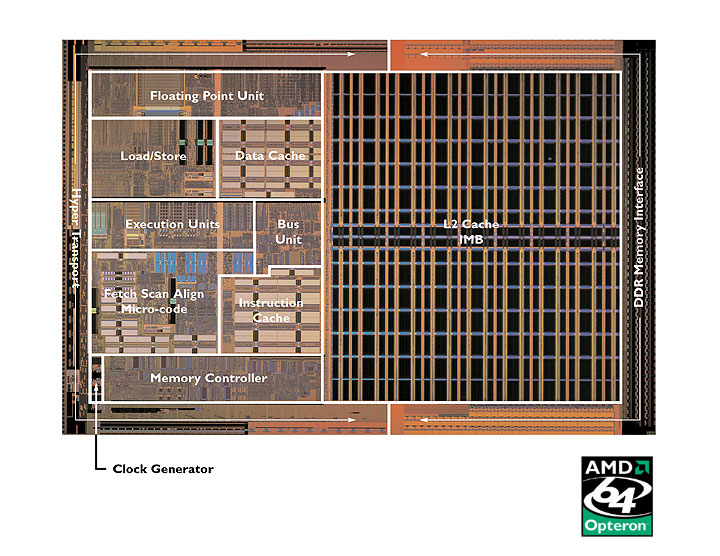
\includegraphics[width=11.25cm]{../caching/Opteron_die_labelled.jpg}};
%\draw[red] (0, 0) grid (9,7);
    \newcommand{\pyrShift}{0.5cm}
\onslide<2->{
    \draw[fill=red,opacity=0.6] (1.9,6.2) rectangle (2.4,5.8);
    \draw[fill=red,opacity=0.6] (1.7,4.2) rectangle (1.9,4.6);

    \begin{scope}[xshift=\pyrShift]
    \draw[fill=red!60!white] (10,7) -- (9.75,6.5) -- (10.25,6.5) -- cycle;
    \node[anchor=west] at (10.1, 6.75) {Registers};
    \end{scope}
}
\onslide<3->{
    %\draw[fill=orange,opacity=0.6] (2.95,2.7) rectangle (4.2,3.6);
    \draw[fill=orange,opacity=0.6] (2.95,2.7) -| (4.2,3.8) -| (3.6,3.65) -- (2.95,3.65) -- (2.95,2.7);
    \draw[fill=orange,opacity=0.6] (2.95,4.6) rectangle (4.2,5.6);

    \begin{scope}[xshift=\pyrShift]
    \draw[fill=orange!60!white] (9.5,6) -- (9.75,6.5) -- (10.25,6.5) -- (10.5,6) -- cycle;
    \node[anchor=west] at (10.35,6.25) {L1 cache};
    \end{scope}
}
\onslide<4->{
    \draw[fill=yellow,opacity=0.6] (4.2,2.1) rectangle (7.9,6.25);
    
    \begin{scope}[xshift=\pyrShift]
    \draw[fill=yellow!60!white] (9.25,5.5) -- (9.5,6) -- (10.5,6) -- (10.75,5.5) -- cycle;
    \node[anchor=west] at (10.6,5.75) {L2 cache};
    \end{scope}
}
\onslide<6->{
    \begin{scope}[xshift=\pyrShift]
    \draw[pattern color=green!60!white,pattern=north west lines] (9.0,5.) -- (9.25,5.5) -- (10.75,5.5) -- (11.,5.) -- cycle;
    \node[anchor=west] at (10.85,5.25) {L3 cache};
    \draw[fill=blue!60!white] (8.5,4.) -- (9.,5.) -- (11,5.) -- (11.5,4.) -- cycle;
    \node[anchor=center,align=center] at (10.,4.5) {main\\memory};
    \end{scope}
}
\onslide<7->{
    \begin{scope}[xshift=\pyrShift]
    \fill[white,opacity=0.9] (7.0,4.5) rectangle (8.4,10.0);
    \begin{scope}[font=\fontsize{10}{11}\selectfont]
        \node[anchor=east] at (9.,6.75) {$<1$ ns};
        \node[anchor=east] at (9.,6.25) {$\sim1$ ns};
        \node[anchor=east] at (9.,5.75) {$\sim5$ ns};
        \node[anchor=east] at (9.,5.25) {$\sim20$ ns};
        \node[anchor=east] at (9.,4.75) {$\sim100$ ns};
    \end{scope}
    \end{scope}
}
\end{tikzpicture}
    \imagecredit{Image: approx 2004 AMD press image of Opteron die; \\ approx register location via chip-architect.org (Hans de Vries)}
\end{frame}

\begin{frame}{cache: real memory}
\begin{tikzpicture}
\node[draw,minimum width=3cm,minimum height=4cm,align=center] (cache) {Data Memory \\ AKA \\ \myemph{L1 Data Cache}};
\draw[Latex-,thick] ([yshift=1cm]cache.west) -- ++(-1cm,0cm) node[left] {address};
\draw[Latex-,thick] ([yshift=-1cm]cache.west) -- ++(-1cm,0cm) node[left] {input (if writing)};
\draw[Latex-] ([yshift=-1.5cm]cache.west) -- ++(-1cm,0cm) node[left,font=\small] {write enable};
\draw[-Latex,thick] ([yshift=1cm]cache.east) -- ++(1cm,0cm) node[right] {value};
\draw[-Latex] ([yshift=-1cm]cache.east) -- ++(1cm,0cm) node[right,font=\small] {\myemph{ready?}};
\begin{visibleenv}<2>
\node[below=1.5cm of cache] (cache2) {L2 Cache};
\draw[dashed,Latex-Latex,very thick] (cache.south) -- (cache2.north);
\end{visibleenv}
\end{tikzpicture}
\end{frame}

\begin{frame}{the place of cache}
% FIXME: picture with CPU, cache, memory
\begin{tikzpicture}
\node[draw,minimum width=1cm,minimum height=2.5cm] (cpu) {CPU};
\node[draw,minimum width=3cm,minimum height=4cm,right=4cm of cpu] (cache) {Cache};
\node[draw,minimum width=1cm,minimum height=6cm,right=4cm of cache,align=center] (mem) {RAM \\ or \\another \\ cache};
\begin{scope}[every node/.style={inner sep=1pt},every pin/.style={align=center,-},every pin edge/.style={-}]
\draw[very thick,-Latex] ([yshift=1cm]cpu.east) -- ([yshift=1cm]cache.west)
    node[midway,pin={north:read {\tt 0xABCD}?\\read {\tt 0x1234}?}] {};
\draw[very thick,Latex-] ([yshift=-1cm]cpu.east) -- ([yshift=-1cm]cache.west)
    node[midway,pin={south:{\tt 0xABCD} is 1000\\{\tt 0x1234} is 4000}] {};
\draw[very thick,-Latex] ([yshift=1cm]cache.east) -- ([yshift=1cm]mem.west)
    node[midway,pin={north:read {\tt 0xABCD}?}] {};
\draw[very thick,Latex-] ([yshift=-1cm]cache.east) -- ([yshift=-1cm]mem.west)
    node[midway,pin={south:{\tt 0xABCD} is 1000}] {};
\end{scope}
% FIXME: hilite hit miss in diagram, seperate into animation
\end{tikzpicture}
\end{frame}

\begin{frame}{memory hierarchy goals}
\begin{itemize}
    \item performance of the fastest (smallest) memory
        \begin{itemize}
            \item hide 100x latency difference? \myemph{99+\% hit (= value found in cache) rate}
        \end{itemize}
    \item capacity of the largest (slowest) memory
\end{itemize}
\end{frame}



\subsection{locality}
\begin{frame}[label=localityIntro]{memory hierarchy assumptions}
\begin{itemize}
    \item \myemph{temporal locality} \\
        ``if a value is accessed now, it will be accessed again soon''
        \begin{itemize}
        \item caches should keep \myemph{recently accessed values}
        \end{itemize}
    \vspace{.5cm}
    \item \myemph{spatial locality} \\
        ``if a value is accessed now, adjacent values will be accessed soon''
        \begin{itemize}
        \item caches should \myemph{store adjacent values at the same time}
        \end{itemize}

    \vspace{1cm}
    \item natural properties of programs --- think about loops
\end{itemize}
\end{frame}

\begin{frame}[fragile,label=localityExamples]{locality examples}
\lstset{language=C,style=small}
\begin{lstlisting}
double computeMean(int length, double *values) {
    double total = 0.0;
    for (int i = 0; i < length; ++i) {
        total += values[i];
    }
    return total / length;
}
\end{lstlisting}
\begin{itemize}
    \item temporal locality: machine code of the loop
    \item spatial locality: machine code of most consecutive instructions
    \item temporal locality: {\tt total}, {\tt i}, {\tt length} accessed repeatedly
    \item spatial locality: {\tt values[i+1]} accessed after {\tt values[i]}
\end{itemize}
\end{frame}


\subsection{typical cache hierarchy}
\usetikzlibrary{arrows.meta,calc,patterns}

\begin{frame}{split caches; multiple cores}
\begin{tikzpicture}
    \tikzset{
        >=Latex,
        connect/.style={<->,ultra thick},
        cache/.style={draw,very thick,align=center},
    }
\node[cache] (icache1) {instr. \\ cache \\ (core 1)};
\node[cache,anchor=west] (dcache1) at ([xshift=2cm]icache1.east) {data \\ cache \\ (core 1)};
\node[cache] (icache2) {instr. \\ cache \\ (core 1)};
\node[cache,anchor=west] (icache2) at ([xshift=3cm]dcache1.east) {instr. \\ cache \\ (core 2)};
\node[cache,anchor=west] (dcache2) at ([xshift=2cm]icache2.east) {data \\ cache \\ (core 2)};
\node[cache, minimum width=4cm,anchor=north] (l21) at ([yshift=-1cm]$(icache1.south)!0.5!(dcache1.south)$) {unified \\ L2 cache \\ (core 1)};
\node[cache, minimum width=4cm,anchor=north] (l22) at ([yshift=-1cm]$(icache2.south)!0.5!(dcache2.south)$) {unified \\ L2 cache \\ (core 2)};
    \node[cache, minimum width=8cm,anchor=north] (l3) at ([yshift=-1cm]$(l21.south)!0.5!(l22.south)$) {L3 cache \\ (shared between cores)};
\foreach \fromC/\toC in {icache1/l21,dcache1/l21,icache2/l22,dcache2/l22,l21/l3,l22/l3} {
\draw[connect] (\fromC.south) -- ++(-0cm,-.5cm) -| (\toC.north);
}
\end{tikzpicture}
\end{frame}

\begin{frame}{hierarchy and instruction/data caches}
    \begin{itemize}
    \item typically separate data and instruction caches for L1
    \vspace{.5cm}
    \item (almost) never going to read instructions as data or vice-versa
    \item avoids instructions evicting data and vice-versa
    \item can optimize instruction cache for different access pattern
    \item easier to build fast caches: that handles less accesses at a time
    \end{itemize}
\end{frame}



\subsection{one-block cache}
\usetikzlibrary{arrows.meta,circuits.logic.US,fit,matrix,positioning,shapes.callouts}

\begin{frame}[fragile,label=buildOneCache]{one-block cache}
\begin{tikzpicture}[remember picture]
\tikzset{
    hi/.style={fill=#1,opacity=0.3,inner sep=1pt}
}
\matrix[tight matrix,
        nodes={font=\small\tt,text width=1.2cm,minimum height=.5cm,inner sep=3pt,inner xsep=0pt},
        row 1/.append style={nodes={font=\small\bfseries,draw=none}},
        column 1/.append style={nodes={visible on=<all:4->,align=center,
            text width=1cm}},
        column 2/.append style={nodes={visible on=<all:6->,align=center}},
        column 3/.append style={nodes={text width=1.5cm,align=center}},
        label={Cache}] (cacheEntries) {
    valid \& tag \& value \\
    \alt<5->{\myemph<5>{1}}{0} \& \alt<5->{\myemph<6>{0101}}{0000} \& \alt<5->{\myemph<5>{AA \myemph<7>{BB}}}{00 00} \\
};
\matrix[tight matrix,label={Memory},
    nodes={font=\small\tt\addfontfeatures{Ligatures=TeX},inner sep=3pt, inner xsep=0pt},
    row 1/.append style={nodes={draw=none,font=\small\bfseries}},
    column 1/.append style={nodes={draw=none,text width=3cm}},
    column 2/.append style={nodes={text width=1.2cm}},
    anchor=north west,
    ] (memory) at ([xshift=1cm]cacheEntries.north east) {
    addresses \& bytes \\
    00000--00001 \& 00 11\\
    00010--00011 \& 22 33 \\
    00100--00101 \& 55 55\\
    00110--00111 \& 66 77 \\
    01000--01001 \& 88 99 \\
    \myemph<6>{0101}0--\myemph<6>{0101}1 \& AA \myemph<7>{BB} \\
    01100--01101 \& CC DD \\
    01110--01111 \& EE FF \\
    10000--10001 \& F0 F1 \\
    \ldots \& |[draw=none]| \ldots\\
};
\begin{visibleenv}<3-9>
    \node[anchor=south west,inner sep=0pt] (readOp1) at ([yshift=2cm]cacheEntries.north west) {read byte at \myemph<6>{0101}\myemph<7>{1}?};
\end{visibleenv}
\begin{visibleenv}<2>
\node[draw=red,anchor=north west,align=left] at ([xshift=.5cm]readOp1.north east){
    decision: divide memory into two-byte blocks \\
    put exactly one of these blocks in the cache
};
\end{visibleenv}
\begin{visibleenv}<4>
    \coordinate (theEntryTop) at ([yshift=-1mm]cacheEntries-2-3.north);
    \node[my callout2=theEntryTop,anchor=west] at ([xshift=1cm]cacheEntries-2-3) {
        is this even a value?
    };
    \node[my callout2=cacheEntries-2-1.center,anchor=west] at ([yshift=-1cm,xshift=0.2cm]cacheEntries-2-1) {
        need \myemph{extra bit} to know
    };
\end{visibleenv}
\begin{visibleenv}<6>
    \coordinate (theEntryTop) at ([yshift=-1mm]cacheEntries-2-3.north);
    \node[my callout2=theEntryTop,anchor=west] at ([yshift=1cm,xshift=1cm]cacheEntries-2-3) {
        value from {\tt 00000, 00010, 00100, \ldots}, or \ldots?
    };
    \node[my callout2=cacheEntries-2-2.south,anchor=west] at ([yshift=-1cm,xshift=-1cm]cacheEntries-2-2) {
        need \myemph{tag} to know
    };
\end{visibleenv}
\begin{visibleenv}<5>
    \node[anchor=north west,inner sep=0pt] at ([yshift=-1mm]readOp1.south west) {invalid, fetch};
\end{visibleenv}
\end{tikzpicture}
\end{frame}


\subsection{direct mapped caches}
\usetikzlibrary{arrows.meta,circuits.logic.US,fit,matrix,positioning,shapes.callouts}
\begin{frame}[fragile,label=buildingCache]{building a (direct-mapped) cache}
\begin{tikzpicture}[remember picture]
\tikzset{
    hi/.style={fill=#1,opacity=0.3,inner sep=1pt}
}
\matrix[tight matrix,
        nodes={font=\small\tt,text width=1.2cm,minimum height=.5cm,inner sep=3pt,inner xsep=0pt},
        row 1/.append style={nodes={font=\small\bfseries,draw=none}},
        column 1/.append style={nodes={draw=none,font=\small\tt,visible on=<all:3->,
            alt=<3>{red}{}}},
        column 2/.append style={nodes={visible on=<all:6->,align=center,
            text width=1cm,
            alt=<6>{red}{}}},
        column 3/.append style={nodes={visible on=<all:8->,align=center}},
        column 4/.append style={nodes={text width=1.5cm,align=center}},
        label={Cache}] (cacheEntries) {
    index \& valid \& tag \& value \\
    00 \& 0 \& 00\& 00 00 \\
    \myemph<all:4>{01} \& \only<all:1-6>{\myemph<all:6>{0}}\only<all:7->{\myemph<all:7>{1}} \& \myemph<all:8>{01} \& \only<all:1-6>{\myemph<all:6>{00 00}}\only<all:7->{\myemph<7>{AA BB}} \\
    10 \& 0 \& 00 \& 00 00 \\
    11 \& 0 \& 00 \& 00 00 \\
};
\matrix[tight matrix,label={Memory},
    nodes={font=\small\tt\addfontfeatures{Ligatures=TeX},inner sep=3pt, inner xsep=0pt},
    row 1/.append style={nodes={draw=none,font=\small\bfseries}},
    column 1/.append style={nodes={draw=none,text width=3cm}},
    column 2/.append style={nodes={text width=1.2cm}},
    anchor=north west,
    ] (memory) at ([xshift=1cm]cacheEntries.north east) {
    addresses \& bytes \\
    00000--00001 \& 00 11\\
    00010--00011 \& 22 33 \\
    00100--00101 \& 55 55\\
    00110--00111 \& 66 77 \\
    01000--01001 \& 88 99 \\
    \myemph<8>{01}010--\myemph<8>{01}011 \& AA \myemph<6-8>{BB} \\
    01100--01101 \& CC DD \\
    01110--01111 \& EE FF \\
    10000--10001 \& F0 F1 \\
    \ldots \& |[draw=none]| \ldots\\
};
\begin{pgfonlayer}{bg}
    \begin{visibleenv}<all:3-4>
        \fill[red,opacity=0.3] ([xshift=\twoZeroes]memory-2-1.north west) rectangle ([xshift=2\twoZeroes]memory-10-1.south west);
        \fill[red,opacity=0.3] ([xshift=4\twoZeroes]memory-2-1.north west) rectangle ([xshift=5\twoZeroes]memory-10-1.south west);
    \end{visibleenv}
\end{pgfonlayer}
\begin{visibleenv}<all:3-5>
    \begin{scope}[dashed,Latex-Latex]
    \foreach \x/\y in {2/2,3/3,4/4,5/5,6/2,7/3,8/4,9/5} {
        \draw (memory-\x-1.west) -- (cacheEntries-\y-4.east);
    }
    \end{scope}
\end{visibleenv}

\begin{pgfonlayer}{bg}
    \begin{visibleenv}<all:3,5>
        \node[fit=(cacheEntries-2-4),hi=green] {};
        \node[fit=(memory-2-2),hi=green] {};
        \node[fit=(memory-6-2),hi=green] {};
        \node[fit=(memory-10-2),hi=green] {};
    \end{visibleenv}
    \begin{visibleenv}<all:4,5,6>
        \node[fit=(cacheEntries-3-4),hi=blue] {};
        \node[fit=(memory-3-2),hi=blue] {};
        \node[fit=(memory-7-2),hi=blue] {};
    \end{visibleenv}
    \begin{visibleenv}<all:5>
        \node[fit=(cacheEntries-4-4),hi=violet] {};
        \node[fit=(memory-4-2),hi=violet] {};
        \node[fit=(memory-8-2),hi=violet] {};
        \node[fit=(cacheEntries-5-4),hi=yellow] {};
        \node[fit=(memory-5-2),hi=yellow] {};
        \node[fit=(memory-9-2),hi=yellow] {};
    \end{visibleenv}

    \begin{visibleenv}<all:8>
        \node[fit=(memory-3-2),hi=blue] {};
        \node[fit=(memory-7-2),hi=blue] {};
    \end{visibleenv}
\end{pgfonlayer}
\begin{visibleenv}<all:2-9>
    \node[anchor=south west,inner sep=0pt] (readOp1) at ([yshift=2cm]cacheEntries.north west) {read byte at 01\myemph<4-5>{01}1?};
\end{visibleenv}
\begin{visibleenv}<all:3-5>
\node[draw=red,anchor=north west,align=left] at ([xshift=.5cm]readOp1.north east){
    exactly \myemph{one place} for each address\\
    spread out what can go in a block
};
\end{visibleenv}
\begin{visibleenv}<all:6>
    \coordinate (theEntryTop) at ([yshift=-1mm]cacheEntries-3-4.north);
    \node[my callout2=theEntryTop,anchor=west] at ([xshift=1cm]cacheEntries-2-4) {
        is this even a value?
    };
    \node[my callout2=cacheEntries-3-2.center,anchor=west] at ([yshift=-1cm,xshift=0.2cm]cacheEntries-2-2) {
        need \myemph{extra bit} to know
    };
\end{visibleenv}
\begin{visibleenv}<all:8>
    \coordinate (theEntryTop) at ([yshift=-1mm]cacheEntries-3-4.north);
    \node[my callout2=theEntryTop,anchor=west] at ([yshift=1cm,xshift=1cm]cacheEntries-2-4) {
        value from {\tt 01010} or {\tt 00010}?
    };
    \node[my callout2=cacheEntries-3-3.south,anchor=west] at ([yshift=-1cm,xshift=-1cm]cacheEntries-3-3) {
        need \myemph{tag} to know
    };
\end{visibleenv}
\begin{visibleenv}<all:7-9>
    \node[anchor=north west,inner sep=0pt] at ([yshift=-1mm]readOp1.south west) {invalid, fetch};
\end{visibleenv}

\node[anchor=north west,align=left] at ([yshift=-0.2cm]cacheEntries.south west) {
    \only<all:1->{cache block: \myemph<1>{2 bytes}} \\
    \only<all:3->{\myemph<3-5>{direct-mapped}} \\
};
\end{tikzpicture}
% FIXME: add storing back fetched value, fetching another value to example
\end{frame}
    
\begin{frame}[fragile,label=cacheOp]{cache operation (read)}
% FIXME: build for this
\begin{tikzpicture}[circuit logic US]
\tikzset{
    myline/.style={-latex,thick},
    myline thin/.style={-latex,thin},
    myline bus/.style={-latex,ultra thick},
    myline no arrow/.style={thick},
    offsetColor/.style={color=yellow!30!black},
    tagColor/.style={color=green!60!black},
    tagColorFill/.style={tagColor,fill=green!60!black},
    dataColor/.style={color=blue!60!black},
    dataColorFill/.style={tagColor,fill=blue!60!black},
    triangle down/.style = {draw,regular polygon, regular polygon sides=3, shape border rotate=180},
}
\matrix[tight matrix,
        nodes={draw,
               font=\small\tt,
               text depth=0.2ex,
               text height=1.4ex,
        },
        row 1/.style={nodes={font=\small\bfseries,draw=none}},
        column 1/.style={nodes={text width=1cm}},
        column 2/.style={nodes={text width=1cm,tagColor}},
        column 3/.style={nodes={draw=none,text width=.5cm}},
        column 4/.style={nodes={text width=3cm,dataColor}},
        ] (cache) {
        valid \& tag \& ~ \&  data \\
    1  \& 10 \& ~ \& 00 11 22 33 \\
    ~ \& ~ \& ~ \& ~\\
    ~ \& ~ \& ~ \& ~\\
    ~ \& ~ \& ~ \& ~\\
    1 \&  11 \& ~ \& B4 B5 B6 B7 \\
    ~ \& ~ \& ~ \& ~\\
    ~ \& ~ \& ~ \& ~\\
    ~ \& ~ \& ~ \& ~\\
};
\begin{scope}[every node/.style={draw,rectangle,dashed,inner xsep=0pt,outer sep=0pt,font=\tt}]
\node (idx) at ([yshift=1cm,xshift=-1cm]cache.north west){100};
\node[left=0cm of idx,tagColor] (tag) {11};
\node[draw=none,left=0cm of tag] {0b};
\node[right=0cm of idx,offsetColor] (offset) {10};
\end{scope}
\draw[thick,dashed,-latex] (idx) |- (cache-6-1.west) node[near start,font=\small,fill=white] {index};

\begin{visibleenv}<2->
    \node[below=0.4cm of cache-9-2,draw,circle,inner sep=3pt] (comp1) {\small =};
    %\coordinate(comp1Intersect) at ($(comp1) + (-.7cm,0.5cm)$);
    %\node[draw,circle,tagColorFill,inner sep=0pt,minimum width=1mm] at (comp1Intersect) {};
    \draw[tagColor,myline] (cache-9-2) -- (comp1);

    %\draw[myline no arrow,tagColor] (tag) |- (comp1Intersect);
    %\draw[myline,tagColor] (comp1Intersect) |- (comp1);
    \draw[tagColor,myline] (tag) |- (comp1) node[near start,font=\small,fill=white] {tag};
    %\draw[myline no arrow,tagColor] (comp1Intersect) |- (comp2Intersect);
    %\draw[myline,tagColor] (comp2Intersect) |- (comp2);

    \node[xshift=.4cm,draw,below=1cm of cache-9-4,and gate,logic gate inputs=nn,label={[font=\scriptsize]center:AND}] (validCheck1) {};

    \draw[myline] (comp1.south) |- (validCheck1.input 1);
    \draw[myline] (cache-9-1.south) |- (validCheck1.input 2);
\end{visibleenv}

\node[fit=(cache-6-1) (cache-6-4),inner sep=1pt,red,draw,line width=3pt] {};

%\node[draw,trapezium,inner xsep=0pt,outer sep=0pt,trapezium angle=75,below=.7cm of validCheck2,
%text width=5cm,shape border rotate=180,xshift=1.5cm] (mux) {};
%\draw[myline] (validCheck1.output) -| (buffer1.west);
%\draw[myline] (cache-9-3.south) -- (buffer1);
%\draw[myline] (buffer1.south) -- (bufEnd1);
\coordinate (outputData) at ([xshift=1cm,yshift=-.3cm]cache-9-4.south east);
\coordinate (beforeOutputData) at ([xshift=-.5cm]outputData);
\coordinate (outputHit) at (outputData |- validCheck1.output);
\begin{visibleenv}<2->
\draw[myline] (validCheck1.output) |- (outputHit) node[right] {is hit? ({\tt 1})};
\end{visibleenv}
\begin{visibleenv}<3->
    \draw[myline no arrow,dataColor] (cache-9-4.south) |- (beforeOutputData);
    \node[draw,mux,anchor=west,inputs=nnnn] (selectByte) at (outputData) {};
    \foreach \x in {1,2,3,4} {
        \draw[dataColor,myline thin] (beforeOutputData) |- (selectByte.input \x);
    };
    \draw[offsetColor,myline] (offset.east) -| (selectByte.north) node[very near start,fill=white,font=\small] {offset};
    \draw[dataColor,myline thin] (selectByte.output) -- ++(0.5cm,0cm) node[right] {data ({\tt B6})};
\end{visibleenv}
\end{tikzpicture}
\end{frame}



\begin{frame}{terminology}
    \begin{itemize}
    \item row = set
        \begin{itemize}
        \item preview: change how much is in a row
        \end{itemize}
    \end{itemize}
\end{frame}

\subsection{tag/index/offset for direct mapped caches}
\usetikzlibrary{decorations.pathreplacing,matrix,shapes.callouts}
\newcommand{\offset}[1]{\textcolor{yellow!30!black}{#1}}
\newcommand{\iindex}[1]{\textcolor{black}{#1}}
\newcommand{\itag}[1]{\textcolor{green!60!black}{#1}}
\begin{frame}{Tag-Index-Offset (TIO)}
\begin{tikzpicture}
\tikzset{
    every matrix/.style={nodes={text width=1.2cm,inner sep=0pt,text height=0.9ex,text depth=.1ex,font=\scriptsize\tt},
        row 1/.append style={nodes={font=\scriptsize\bfseries,draw=none}},},
    every label/.style={label distance=-2mm,font=\small},
    offsetColor/.style={color=yellow!30!black},
    tagColor/.style={color=green!60!black},
    tagColorFill/.style={tagColor,fill=green!60!black},
    dataColor/.style={color=blue!60!black},
    dataColorFill/.style={tagColor,fill=blue!60!black},
}
\matrix[tight matrix,
        column 1/.append style={nodes={draw=none}},
        column 2/.append style={nodes={align=center,text width=1cm}},
        column 3/.append style={nodes={align=center,tagColor}},
        column 4/.append style={nodes={text width=1.5cm,align=center,dataColor}},
        label={\myemph<2>{$2$ byte blocks}, $4$ sets}] (cache1) at (0,0) {
    index \& valid \& tag \& value \\
    00 \& 1 \& 000\& 00 11 \\
    01 \& 1 \& 001 \& AA BB \\
    10 \& 0 \& -- \& -- -- \\
    11 \& 1 \& 001 \& EE \myemph{FF} \\
};
\matrix[tight matrix,anchor=north west,
        column 1/.append style={nodes={draw=none}},
        column 2/.append style={nodes={align=center,text width=1cm}},
        column 3/.append style={nodes={align=center,tagColor}},
        column 4/.append style={nodes={text width=3cm,align=center,dataColor}},
        label={$4$ byte blocks, $2$ sets}] (cache2) at ([yshift=-0.5cm]cache1.south west){
    index \& valid \& tag \& value \\
    0 \& 1 \& 000 \& 00 11 22 33\\
    1 \& 1 \& 001 \& CC DD EE \myemph{FF}\\
};

\matrix[tight matrix,anchor=north west,
        column 1/.append style={nodes={draw=none}},
        column 2/.append style={nodes={align=center,text width=1cm}},
        column 3/.append style={nodes={align=center,tagColor}},
        column 4/.append style={nodes={text width=1.5cm,align=center,dataColor}},
        label={$2$ byte blocks, $8$ sets}] (cache3) at ([xshift=1.8cm]cache1.north east) {
    index \& valid \& tag \& value \\
    000 \& 1 \& 00 \& 00 11 \\
    001 \& 1 \& 01 \& F1 F2 \\
    010 \& 0 \& -- \& -- -- \\
    011 \& 0 \& -- \& -- -- \\
    100 \& 0 \& -- \& -- -- \\
    101 \& 1 \& 00 \& AA BB \\
    110 \& 0 \& -- \& -- -- \\
    111 \& 1 \& 00 \& EE \myemph{FF} \\
};
\node[anchor=south west,align=left] (example1) at ([yshift=0.5cm]cache1.north west) {
    address {\tt 0011\myemph<3>{1\myemph<2>{1}}} (stores value {\tt 0xFF}) \\
    \begin{tabular}{llll}
    cache & tag & index & offset \\\hline
    \myemph<2>{2 byte blocks}, \myemph<4>{4 sets} &
    \only<0|handout:0>{???}\only<7->{\itag{001}} &
    \only<0|handout:0>{???}\only<4->{\iindex{11}} &
    \only<0|handout:0>{???}\only<2->{\offset{1}} \\
    \myemph<2>{2 byte blocks}, \myemph<4>{8 sets} &
    \only<0|handout:0>{???}\only<7->{\itag{00}} &
    \only<0|handout:0>{???}\only<5->{\iindex{111}} &
    \only<0|handout:0>{???}\only<2->{\offset{1}} \\
    \myemph<3>{4 byte blocks}, \myemph<4>{2 sets} &
    \only<0|handout:0>{???}\only<7->{\itag{001}} &
    \only<0|handout:0>{???}\only<4->{\iindex{1}} &
    \only<0|handout:0>{???}\only<3->{\offset{11}}\\
    \end{tabular}
};
\tikzset{
    tBox/.style={fill=white,align=left,draw=red,rectangle,line width=2pt,anchor=north west,at=(example1.south west)},
}
\begin{visibleenv}<2|handout:0>
    \node[my callout2={cache1-2-4.east},align=left] at ([xshift=0.5cm,yshift=0.5cm]cache1-2-4.east) {
        $2=2^1$ bytes in block \\ 1 bit to say which byte
    };
\end{visibleenv}
\begin{visibleenv}<3|handout:0>
    \node[my callout2={cache2-2-4.north},align=left,anchor=south] at ([yshift=0.5cm]cache2-2-4.north) {
        $4=2^2$ bytes in block \\ 2 bits to say which byte
    };
\end{visibleenv}
\begin{visibleenv}<4|handout:0>
    \draw[decorate,decoration={brace,amplitude=10pt},thick,xshift=4pt]  (cache1-2-4.north east) -- (cache1.south east);
    \coordinate (decorationEnd1) at ([xshift=14pt]$(cache1-2-4.north east)!0.5!(cache1.south east)$);
    \node[my callout2=decorationEnd1,anchor=west,align=left] at ([xshift=.5cm]decorationEnd1) {
        $2^2 = 4$ sets \\
        \myemph{2 bits} to index set
    };
\end{visibleenv}
\begin{visibleenv}<5|handout:0>
    \draw[decorate,decoration={brace,amplitude=10pt,mirror},thick,xshift=-4pt]  (cache3-2-1.north west) -- (cache3.south west);
    \coordinate (decorationEnd2) at ([xshift=-14pt]$(cache3-2-1.north west)!0.5!(cache3.south west)$);
    \node[my callout2=decorationEnd2,anchor=east,align=left] at ([xshift=-.5cm]decorationEnd2) {
        $2^3 = 8$ sets \\
        \myemph{3 bits} to index set
    };
\end{visibleenv}
\begin{visibleenv}<6|handout:0>
    \node[my callout2=cache2.east,anchor=west,align=left] at ([yshift=1cm,xshift=.5cm]cache2.east) {
        $2^1 = 2$ sets \\
        \myemph{1 bit} to index set
    };
\end{visibleenv}
\begin{visibleenv}<7|handout:0>
    \node[tBox] {
        \myemph{tag} --- whatever is left over
    };
\end{visibleenv}
\end{tikzpicture}
\end{frame}

\begin{frame}{Tag-Index-Offset formulas (direct-mapped only)}
\def\arraystretch{1.5}
\begin{tabular}{ll}
$m$ & memory addreses bits (Y86-64: 64) \\
$S=2^s$ & number of sets \\
$s$  & (set) index bits \\
$B=2^b$ & block size \\
$b$ & (block) offset bits \\
$t = m - (s+b)$ & tag bits \\
$C = B \times S$ & cache size (if direct-mapped) \\
\end{tabular}
\end{frame}


\subsubsection{aside: cache size}
\begin{frame}{cache size}
    \begin{itemize}
    \item cache size = amount of \textit{data} in cache
    \item not included metadata (tags, valid bits, etc.)
    \end{itemize}
\end{frame}

\subsection{prelim. formulas}
\begin{frame}{Tag-Index-Offset formulas (direct-mapped)}
\begin{itemize}
\item (formulas derivable from prior slides)
\end{itemize}
\def\arraystretch{1.5}
\begin{tabular}{ll}
$S=2^s$ & number of sets \\
$s$  & (set) index bits \\
$B=2^b$ & block size \\
$b$ & (block) offset bits \\
$m$ & memory addreses bits \\
$t = m - (s+b)$ & tag bits \\
$C = B \times S$ & \myemph<2>{cache size} (if direct-mapped) \\
\end{tabular}
\end{frame}


\subsection{tio for DM: exercise}
\input{../caching/tioDmExercise}

\subsection{simulating a direct mapped cache}
\usetikzlibrary{matrix,shapes.callouts}
\begin{frame}<1-12>[fragile,label=pattern1]{example access pattern (1)}
\begin{tikzpicture}
\tikzset{
    v/.style={visible on=<#1->,alt=<#1>{red}},
    h/.style={alt=<#1>{red}},
}
\tikzset{
    tagColor/.style={color=green!60!black},
    dataColor/.style={color=blue!60!black},
    offsetColor/.style={color=yellow!30!black},
}
\matrix[tight matrix,
        nodes={font=\small,minimum height=.5cm,text depth=.1ex},
        column 1/.append style={nodes={font=\small\tt,text width=3.3cm,align=left}},
        row 1/.append style={nodes={font=\small\bfseries}},
        column 2/.append style={nodes={text width=1.3cm}},
        ] (pattern) {
    address (hex)\& result \\
    00000000 (00) \& |[v=4]| miss \\
    00000001 (01) \& |[v=5,h=12]| hit \\
    01100011 (63) \& |[v=6]| miss \\
    01100001 (61) \& |[v=7,h=12]| miss \\
    01100010 (62) \& |[v=8]| hit \\
    00000000 (00) \& |[v=9,h=12]| miss \\
    01100100 (64) \& |[v=10]| miss \\
};
\begin{pgfonlayer}{fg}
    \begin{visibleenv}<12-13>
        \node[my callout2=pattern-7-2.east,anchor=west] at ([xshift=1cm]pattern-7-2.east) {
            miss caused by \myemph{conflict}
        };
    \end{visibleenv}
\end{pgfonlayer}
\matrix[tight matrix,anchor=north west,
        nodes={font=\small\tt,text depth=.1ex,text height=1ex,minimum height=1cm},
        row 1/.append style={nodes={font=\small\bfseries,minimum height=.5cm}},
        column 1/.append style={nodes={draw=none,text width=1.2cm}},
        column 2/.append style={nodes={align=center,text width=1cm}},
        column 3/.append style={nodes={align=center,tagColor,text width=1.5cm}},
        column 4/.append style={nodes={text width=2.5cm,align=center,dataColor,
            text depth=2.3ex}},
        row 1 column 4/.append style={nodes={text depth=.1ex}},
        label={[font=\small]$2$ byte blocks, $4$ sets}] (cache) at ([xshift=.5cm]pattern.north east) {
    index \& valid \& tag \& value \\
    00 \& \zzx{1}{3}{0}\z{4}{1} \& \zz{4,5}{6}{00000}\zz{7}{8}{01100}\z{9}{00000} \& 
        \zz{4,5}{6}{mem[0x00] mem[0x01]}%
        \zz{7}{8}{mem[0x60] mem[0x61]}%
        \z{9}{mem[0x00] mem[0x01]}%
        \\
    01 \& \zzx{1}{5}{0}\z{6}{1} \& \z{6}{01100} \& \z{6}{mem[0x62] mem[0x63]} \\
    10 \& \zzx{1}{9}{0}\z{10}{1} \& \z{10}{01100} \& \z{10}{mem[0x64] mem[0x65]} \\
    11 \& 0 \& ~ \& ~ \\
};
\begin{visibleenv}<2->
    \node[anchor=north west,font=\small,align=left] (explain1) at ([yshift=-.5cm]pattern.south west) {
        $B=2=2^b$ byte block size \\
        $b=\myemph<2>{1}$ (block) offset bits \\
        $S=4=2^s$ sets \\
        $s=\myemph<2>{2}$ (set) index bits \\
    };
    \node[anchor=north west,font=\small,align=left] (explain2) at ([xshift=.5cm]explain1.north east) {
        $m = 8$ bit addresses \\ 
        $t = m - (s+b) = \myemph<2>{5}$ tag bits\\
    };
\end{visibleenv}
\begin{visibleenv}<3->
    \coordinate (tagTopLeft) at ([xshift=.1ex]pattern-2-1.north west);
    \coordinate (tagBottomLeft) at ([xshift=.1ex]pattern-8-1.south west);
    \coordinate (indexTopLeft) at ([xshift=5\oneZero]tagTopLeft);
    \coordinate (offsetTopLeft) at ([xshift=2\oneZero]indexTopLeft);
    \coordinate (offsetTopRight) at ([xshift=1\oneZero]offsetTopLeft);
    \coordinate (tagBottomRight) at (tagBottomLeft -| indexTopLeft);
    \coordinate (indexBottomRight) at (tagBottomLeft -| offsetTopLeft);
    \coordinate (offsetBottomRight) at (tagBottomLeft -| offsetTopRight);
    \fill[tagColor,opacity=0.3] (tagTopLeft) rectangle (tagBottomRight);
    \fill[offsetColor,opacity=0.3] (offsetTopLeft) rectangle (offsetBottomRight);
    \begin{scope}[every node/.style={anchor=north,text depth=.2ex,text height=1ex}]
        \node[tagColor,xshift=-.5cm] at ($(tagBottomLeft)!.5!(tagBottomRight)$) {
            tag
        };
        \node[xshift=-.2cm] at ($(tagBottomRight)!.5!(indexBottomRight)$) {
            index
        };
        \node[offsetColor,xshift=.6cm] at ($(indexBottomRight)!.5!(offsetBottomRight)$) {
            offset
        };
    \end{scope}
\end{visibleenv}

\end{tikzpicture}
\end{frame}


\subsection{exercise: direct-mapped cache access}
\begin{frame}[fragile,label=pattern1Ex]{exercise}
\begin{tikzpicture}
\tikzset{
    v/.style={visible on=<#1->,alt=<#1>{red}},
    h/.style={alt=<#1>{red}},
}
\tikzset{
    tagColor/.style={color=green!60!black},
    dataColor/.style={color=blue!60!black},
    offsetColor/.style={color=yellow!30!black},
}
\matrix[tight matrix,
        nodes={font=\small,minimum height=.5cm,text depth=.1ex},
        column 1/.append style={nodes={font=\small\tt,text width=3.3cm,align=left}},
        row 1/.append style={nodes={font=\small\bfseries}},
        column 2/.append style={nodes={text width=1.3cm}},
        ] (pattern) {
    address (hex)\& result \\
    00000000 (00) \& ~ \\
    00000001 (01) \& ~ \\
    01100011 (63) \& ~ \\
    01100001 (61) \& ~ \\
    01100010 (62) \& ~ \\
    00000000 (00) \& ~ \\
    01100100 (64) \& ~ \\
};
\matrix[tight matrix,anchor=north west,
        nodes={font=\small\tt,text depth=.1ex,text height=1ex,minimum height=1cm},
        row 1/.append style={nodes={font=\small\bfseries,minimum height=.5cm}},
        column 1/.append style={nodes={draw=none,text width=1.2cm}},
        column 2/.append style={nodes={align=center,text width=1cm}},
        column 3/.append style={nodes={align=center,tagColor,text width=1.5cm}},
        column 4/.append style={nodes={text width=5cm,align=center,dataColor,
            text depth=2.3ex}},
        row 1 column 4/.append style={nodes={text depth=.1ex}},
        label={[font=\small]$4$ byte blocks, $4$ sets}] (cache) at ([xshift=.5cm]pattern.north east) {
    index \& valid \& tag \& value \\
    00 \& ~ \& ~ \& ~ \\
    01 \& ~ \& ~ \& ~ \\
    10 \& ~ \& ~ \& ~ \\
    11 \& ~ \& ~ \& ~ \\
};
\begin{visibleenv}<2>
    \node[draw=red,very thick,anchor=north west,align=left] (ex1) at ([yshift=-.5cm]pattern.south west) {
        how is the 8-bit address 61 (01100001) split \\ 
        up into tag/index/offset? 
    };
    \node[anchor=north west,align=left,font=\small] at (ex1.north east) {
        $b$ block offset bits;\\
        $B=2^b$ byte block size; \\
        $s$ set index bits; $S=2^s$ sets ;\\
        $t=m-(s+b)$ tag bits (leftover)
    };
\end{visibleenv}
\begin{visibleenv}<3-4>
\iftoggle{heldback}{}{
    \node[anchor=north west,font=\small,align=left] (explain1) at ([yshift=-.5cm]pattern.south west) {
        $m = 8$ bit addresses \\ 
        $S=4=2^s$ sets \\
        $s=\myemph<2>{2}$ (set) index bits \\
    };
    \node[anchor=north west,font=\small,align=left] (explain2) at ([xshift=.5cm]explain1.north east) {
        $B=4=2^b$ byte block size \\
        $b=\myemph<2>{2}$ (block) offset bits \\
        $t = m - (s+b) = \myemph<2>{4}$ tag bits\\
    };
}
\end{visibleenv}
\begin{visibleenv}<5>
    \node[anchor=north west,draw=red,very thick,align=left] at ([yshift=-.5cm]pattern.south west) {
        exercise: which accesses are hits?
    };
\end{visibleenv}
\begin{visibleenv}<4->
\iftoggle{heldback}{}{
    \coordinate (tagTopLeft) at ([xshift=.1ex]pattern-2-1.north west);
    \coordinate (tagBottomLeft) at ([xshift=.1ex]pattern-8-1.south west);
    \coordinate (indexTopLeft) at ([xshift=4\oneZero]tagTopLeft);
    \coordinate (offsetTopLeft) at ([xshift=2\oneZero]indexTopLeft);
    \coordinate (offsetTopRight) at ([xshift=2\oneZero]offsetTopLeft);
    \coordinate (tagBottomRight) at (tagBottomLeft -| indexTopLeft);
    \coordinate (indexBottomRight) at (tagBottomLeft -| offsetTopLeft);
    \coordinate (offsetBottomRight) at (tagBottomLeft -| offsetTopRight);
    \fill[tagColor,opacity=0.3] (tagTopLeft) rectangle (tagBottomRight);
    \fill[offsetColor,opacity=0.3] (offsetTopLeft) rectangle (offsetBottomRight);
    \begin{scope}[every node/.style={anchor=north,text depth=.2ex,text height=1ex}]
        \node[tagColor,xshift=-.5cm] at ($(tagBottomLeft)!.5!(tagBottomRight)$) {
            tag
        };
        \node[xshift=-.2cm] at ($(tagBottomRight)!.5!(indexBottomRight)$) {
            index
        };
        \node[offsetColor,xshift=.6cm] at ($(indexBottomRight)!.5!(offsetBottomRight)$) {
            offset
        };
    \end{scope}
}
\end{visibleenv}
\end{tikzpicture}
\end{frame}


\subsection{mapping misses to sets (DM)}
\usetikzlibrary{arrows.meta}

\begin{frame}{mapping of sets to memory (direct-mapped)}
\begin{tikzpicture}
    \tikzset{
    >=Latex,
        cache/.style={draw,very thick},
        set 0/.style={draw,thin,fill=blue!20},
        set K/.style={draw,thin,fill=orange!30},
    }
\node[anchor=south] at (.5, 2) { DM cache };
\draw[cache] (0, 0) rectangle ++(1, 2);
\draw[set 0] (0, 1.9) rectangle ++(1, 0.1);
\draw[<-,thick] (0, 1.95) -- ++(-.5cm, 0cm) node[left] {set 0};
\draw[set K] (0, 0.4) rectangle ++(1, 0.1);
\draw[<-,thick] (0, 0.45) -- ++(-.5cm, 0cm) node[left] {set $K$};
\begin{visibleenv}<2>
\draw[<->,very thick] (1.25, 2) -- ++(0, -2);
\end{visibleenv}
\begin{scope}[xshift=3cm]
\node[anchor=south] at (.5, 2) { memory };
\draw[cache] (0, -6) rectangle ++(1, +8);
\draw[set 0] (0, 1.9) rectangle ++(1, 0.1);
\draw[set 0] (0, -.1) rectangle ++(1, 0.1);
\draw[set 0] (0, -2.1) rectangle ++(1, 0.1);
\draw[set 0] (0, -4.1) rectangle ++(1, 0.1);
\draw[set K] (0, 0.4) rectangle ++(1, 0.1);
\draw[set K] (0, -1.6) rectangle ++(1, 0.1);
\draw[set K] (0, -3.6) rectangle ++(1, 0.1);
\draw[set K] (0, -5.6) rectangle ++(1, 0.1);
\begin{visibleenv}<2>
\draw[<->,very thick] (1.25, 1.9) -- ++(0, -2) node[midway,right,align=left] {
    values which would be stored in same set \\
    (cache size) bytes apart
};
\end{visibleenv}
\begin{visibleenv}<3>
\draw[<-] (1.0, -.05) -- ++ (1, 0) node[right] {array[0] here};
\draw[<-] (1.0, -1.55) -- ++ (1, 0) node[right,align=left] {array[X] where \\
    X = K \cdot (array elements per cache block)
};
\end{visibleenv}
\begin{visibleenv}<4>
\draw[<-] (1.0, -.05) -- ++ (1, 0) node[right] {array[0] here};
    \draw[<-] (1.0, -2.05) -- ++ (1, 0) node[right,align=left] (cache by array elem) {array[X] \\
    X = (cache size / array element size)
};
\node[anchor=north,draw=red,align=left,very thick] at (cache by array elem.south) {
    elements (cache size) bytes apart in array \\
    beware conflict misses!
};
\end{visibleenv}
\end{scope}
\end{tikzpicture}
\end{frame}


\section{backup slides}
\begin{frame}{backup slides}
\end{frame}

\end{document}
